\documentclass[letterpaper,12pt,oneside]{book}
%\usepackage[a4paper,includeall,bindingoffset=0cm,margin=2cm,marginparsep=0cm,marginparwidth=0cm]{geometry}
\usepackage[top=1in, left=0.9in, right=1.25in, bottom=1in]{geometry}
\usepackage{ThesisMartinIPN}
\usepackage[utf8]{inputenc}
\usepackage{url}
\usepackage[T1]{fontenc}
\usepackage[spanish,es-nodecimaldot,es-tabla]{babel}
\usepackage{graphicx}
\usepackage{tikz}
\usepackage{tocloft}
\graphicspath{{./figs/}}
\usepackage{setspace}
\usepackage{comment}
\usepackage{hyperref}
\usepackage{slashed}
\usepackage{amsmath}
\usepackage{caption}
\usepackage{subcaption}

\usepackage{ifoddpage}

\urlstyle{same}
\usepackage[titletoc]{appendix}

\hypersetup{
   colorlinks=true,
   urlcolor=cyan,
   linkcolor=black,
   citecolor=black,
   filecolor=magenta,
   pdftitle={Sharelatex Example},
   pdfpagemode=FullScreen,
}
\usepackage[style=numeric, sorting=none]{biblatex}
\addbibresource{sample.bib}
%\usepackage[natbibapa]{apacite}
%\usepackage[round]{natbib}

%\renewcommand\cftsecpresnum{\S}
%\renewcommand\cftsubsecpresnum{\S}

%%%%%%%%%%%%%%%%%%%%%%%%%%%%%

% Modificación de la plantilla original de esta url: 
% https://es.overleaf.com/latex/templates/tesis-unam-ingenieria-energia/kfffjrxcckdp

% Adaptada por Martin Moreno Guzmán para el CICATA-IPN.
% Cualquier sugerencia, corrección o comentario a: mmorenog1500@alumno.ipn.mx

% A continuación los comentarios de la plantilla original:

% Comparto una plantilla para la PORTADA que use en mi tesis
% Modificar el archivo de portada. tex

\setlength{\parindent}{1em}
\setlength{\parskip}{1em}
\renewcommand{\baselinestretch}{1.2}
%\usepackage{biblatex}
\usepackage{feynmp}
\DeclareGraphicsRule{*}{mps}{*}{}

\usepackage{tikz-feynman}
\tikzfeynmanset{compat=1.1.0}


\begin{document}

\frontmatter
\begin{titlepage}
  \thispagestyle{empty}
  \begin{minipage}[c][0.17\textheight][c]{0.25\textwidth}
    \begin{center}
    \hspace*{-13mm}
      \includegraphics[ height=5cm]{Images/Cinvestav.jpg}
    \end{center}
  \end{minipage}
  \begin{minipage}[c][0.195\textheight][t]{0.75\textwidth}
    \begin{center}
      \vspace{0.3cm}
             {\color{black}\textsc{\large Centro de Investigación y de Estudios Avanzados del Instituto Politécnico Nacional} }\\[0.5cm]
             \vspace{0.3cm}
                    {\color{black}\hrule height3pt}
                    \vspace{.2cm}
                           {\color{black}\hrule height2pt}
                           \vspace{.8cm}
                           \textsc{ \large CINVESTAV}\\[0cm] %
    \end{center}
  \end{minipage}
  \begin{minipage}[c][0.81\textheight][t]{0.25\textwidth}
    \vspace*{5mm}
    \begin{center}
      \hskip0.5mm
             %{\color{purple}\vrule width1pt height13cm }
             \vspace{5mm}
             \hskip2pt
                 {\color{black}\vrule width3pt height13cm}
                 \hskip2mm
                     {\color{black}\vrule width1pt height13cm} \\
                     \vspace{5mm}
                     \hspace*{1mm}
                     \includegraphics[height=4cm]{Images/}
    \end{center}
  \end{minipage}
  \begin{minipage}[c][0.81\textheight][t]{0.75\textwidth}
    \begin{center}
      \vspace{1cm}

      {\color{black}{\large\scshape Medición de la masa del Leptón tau en estados finales semi-invisibles en topología 1x1 en la colaboración Belle II}}\\[.2in]

      \vspace{1cm}            

      \textsc{\LARGE T\hspace{0.5cm}E\hspace{0.5cm}S\hspace{0.5cm}I\hspace{0.5cm}S}\\[1.5cm]
      \textsc{\large que para obtener el grado de:}\\[0.5cm]
      \textsc{\large Maestría en Ciencias en la Especialidad de Física}\\[0.5cm]
      
      {\color{black}\textsc{\large p r e s e n t a:}}\\[0.5cm]
      \textsc{\large {Johan Andrés Colorado Caicedo}}\\[1cm]          

      \vspace{0.5cm}

      {\large\scshape 
        {\color{black}Director de tesis}\\[0.3cm] {Dr. Eduard de la Cruz Burelo \\ 
          }}\\[.2in]

      \vspace{0.5cm}
       
      \large{CDMX, Septiembre 2021}
    \end{center}
  \end{minipage}
\end{titlepage}
%---------------------------------
\tableofcontents
\newpage
\listoffigures
\chapter{Agradecimientos}

Quiero agradecer la confianza, el apoyo, la guía y la enseñanza ardúa brindada por el Dr. Eduard De La Cruz Burelo a quién por fortuna tuve como asesor y profesor. A mis sinodales los doctores, Pablo Roig Garcés y Heriberto Castilla Valdez quienes con sus observaciones ayudaron a mejorar esta tesis. A mis compañeros por las reuniones tan enriquecedoras y por último al CONACYT y al CINVESTAV por la oportunidad que me brindaron para continuar con mis estudios posgraduales y el apoyo económico dado.

\newpage


\chapter{Resumen}

En esta tesis se determina la masa del leptón tau por medio de la comparación de tres métodos para decaimientos con estados finales semi-invisibles.
La medición fue realizada para el decaimiento \(\tau\rightarrow\pi\nu\) (señal). Se obtiene que el mejor resultado fue brindado por el método \(M_{min}\) para una masa del leptón tau de \(m_{\tau}=1777.06\pm0.44\) MeV. La medición se completó usando datos oficiales de Monte Carlo de la colaboración Belle II en la campaña MC13a finalizada en el año 2020.

  


\newpage


\chapter{Abstract}

In this thesis, the mass of the tau lepton is determined by comparing three methods for decays with semi-invisible final states.
The measurement was performed for the decay \(\tau \rightarrow \pi \nu \) (signal). It is obtained that the best result was provided by the method \(M_{min}\) for a mass of the tau lepton of \(m _{\tau} = 1777.06 \pm 0.44\) MeV. The measurement was completed using official Monte Carlo data from the Belle II collaboration in the MC13a campaign ended in 2020. 



\mainmatter

\chapter{Introducción}

En los intentos del ser humano para comprender de qué está hecho el universo, se han llegado a avances mayúsculos, como el descubrimiento del Bosón de Higgs en 2012 \cite{Chatrchyan_2012} que da una explicación (aunque aún no del todo completa) al problema anacrónico de la masa, ya que es el campo de Higgs quien dota de masa a los leptones a través de la interacción de Yukawa, esto según el Modelo Estándar de Partículas Elementales (SM), pero aún continúa siendo un misterio qué mecanismo le da masa al mismo bosón de Higgs o también a los neutrinos, que se ha comprobado que tienen una masa debido a su propia oscilación, esto descubierto por Takaaki Kajita y Arthur B. McDonald. Lo anterior nos indica que hay indicios que el SM no está completo o que debe haber física más allá del modelo estándar (BSM), es por esto que resulta interesante y de alta relevancia estudiar propiedades de las diferentes partículas elementales.


En miras de proseguir en el entendimiento del misterio sobre ``¿de qué estamos hechos?'', surge como consecuencia de darle una interpretación a las soluciones de la ecuación de Dirac la existencia de un tipo de materia con algunas propiedades completamente opuestas como lo es la antimateria, i.e, una partícula y su antipartícula (por ejemplo el protón y el antiprotón) tienen la misma masa, pero carga eléctrica de signo opuesto, de igual manera que algunos números cuánticos. 

En la era de la radiación, instantes luego de la gran explosión habían sólo fotones en el universo, a medida que este se fue enfriando tales fotones debieron decaer en pares de partícula-antipartícula, esto nos puede llevar a pensar que en el universo debe haber la misma cantidad de ambas sustancias (materia y antimateria), pero si es así, ¿por qué lo que conocemos y hasta nosotros mismos estamos hechos de materia ordinaria y no de su contraparte?. Este problema recibe el nombre de bariogénesis, donde se reúnen los procesos hipotéticos mediante los cuales se produjo la asimetría entre bariones y antibariones (partículas conformadas por tres quarks) durante los primeros instantes de vida del universo, resultando en cantidades elevadas de materia ordinaria residual en el universo actual. Esta resulta ser una gran motivación para que los grandes experimentos alrededor del mundo, entre ellos Belle, quien con cierto grado de éxito trató de darle respuesta a este gran interrogante encontrando que en el sector de los mesones B existe una diferencia entre materia y antimateria en condiciones similares al comienzo del universo: La llamada violación CP (primero medida en partículas llamadas Kaones en 1964) descrita por el mecanismo de Kobayashi-Maskawa \cite{Kobayashi:1973fv}, trabajo por el cual recibieron el premio Nobel de física en el año 2008 luego de los resultados del experimento anteriormente mencionado. Pero esto no es suficiente, dicha diferencia no es sustancial para dar explicación a la asimetría materia-antimateria, es por esta razón que se han hecho mayores apuestas que se ven reflejadas en una actualización no sólo estructural, sino de software y poder de cómputo, tanto en el acelerador KEKB que ahora pasó a ser SuperKEKB que es un acelerador de leptones de 3016 m de perímetro donde circulan electrones a una energía de 7 GeV en un sentido y positrones a una energía de 4 GeV en el sentido opuesto, estos haces chocan en un punto a una energía del centro de momentos de aproximadamente 10.58 GeV que corresponde a la energía de la resonancia \(\Upsilon (4S)\), ahí, en este punto se encuentra ubicado el detector Belle II (actualización del detector Belle). Entre las mejoras de la actualización se encuentra una mayor luminosidad instantánea, un mejor sistema de triggers, que en conjunto hacen que Belle II pueda tomar datos unas 40 veces más rápido que su predecesor. Al contar con más estadística, también mejores sistemas de trigger y software en general, se prevé que podrían existir las condiciones necesarias para encontrar física BSM, de ser así, podríamos muy prontamente responder el por qué de tal asimetría y otras cuestiones de gran relevancia en la física actual.

Es importante para poder llegar a encontrar resultados de nueva física en el marco del nuevo experimento Belle II primero confirmar o validar resultados del SM, de modo que sea factible llegar a resultados más precisos al realizar mediciones de parámetros y/o procesos bien conocidos. También, poder de esta manera identificar partículas, hallar nuevas o estudiar procesos que contengan ese toque de nueva física tan buscada en la actualidad. Es en este punto donde entra en acción el grupo de física de altas energías (HEP) del CINVESTAV que trabaja en la colaboración internacional Belle II, desde donde en particular se hacen aportaciones en la física del tau. Estudiar el leptón tau es de gran importancia, porque esta partícula es muy sensible a la nueva física debido a algunas características peculiares, entre ellas, que es el leptón más masivo de las tres familias y que tiene una vida corta. Estas características hacen del leptón tau una partícula difícil de detectar y con muchos canales de decaimiento; esta partícula es 1.500 veces más pesada que un electrón, pero tiene la misma carga y los mismos números cuánticos, exceptuando el sabor leptónico.
La gran masa del tau abre la posibilidad de estudiar muchos modos de desintegración cinemáticamente permitidos y extraer información dinámica relevante de allí. Que el leptón tau sea el más masivo de las tres familias y que este sea el único de los leptones que puede decaer en hadrones incentiva que la física del tau sea un laboratorio extraordinario  para estudiar la cromodinámica cuántica (QCD), ya que los hadrones son partículas compuestas, además de ser el leptón que nos proporciona un marco de estudio completo para la electrodinámica cuántica (QED). También en las desintegraciones del leptón tau se podrían encontrar violaciones de las leyes de conservación, como por ejemplo, la violación de carga-paridad (CPV), situación que está muy relacionada con el momento dipolar eléctrico (EDM) del tau. A través de procesos de desintegración que no están considerados dentro del modelo estándar (SM) y que tienen al leptón tau como protagonista se podrían alcanzar los próximos resultados de gran impacto en la comunidad, es por estas razones que la física del tau es de suma importancia en la física de partículas actual. Con estos ambiciosos propósitos en movimiento debemos asegurarnos de que el experimento sea capaz de detectar partículas y también que seamos capaces de reconstruir procesos que son bien conocidos y es por medio de mediciones de diferentes parámetros como la masa de las partículas que esto se logra. Estos procesos son los del SM y mediante estos podemos determinar con mayor precisión parámetros predichos teóricamente y medidos en grandes experimentos previamente. Por ejemplo, la mejor medida de la masa de la tau fue realizada por la colaboración BESIII \cite{PhysRevD.90.012001} (PDG) en 2014, seguidos por BaBar \cite{Aubert_2009} en 2009 y por Belle \cite{PhysRevLett.99.011801} en 2007.


La masa de los quarks y leptones son parámetros fundamentales en el SM, en esta tesis se propone usar un nuevo método para la medición de la masa del leptón tau tomando un canal de decaimiento que hasta el momento no ha sido utilizado en la colaboración Belle II debido a inconvenientes de carácter técnico que se presentan al momento de detectar las partículas de tal decaimiento, ya que tenemos en este partículas invisibles para nuestros detectores, también los métodos hasta ahora usados para medir la masa del tau como el método ARGUS ha usado topologías diferentes \cite{Albrecht1995}. El método de ARGUS es un método de pseudo-masa que considera algunas aproximaciones cinemáticas, como por ejemplo, asumir masa cero del neutrino del tau, aproximar la dirección de vuelo del tau a la de las tres partículas cargadas y tomar la energía del tau como la mitad de la energía del centro de masa. Como cada tau involucra una partícula perdida (neutrino) y además por el tiempo de vida tan corto del tau que lo hace indetectable, esto hace que con el método ARGUS sea imposible la reconstrucción completa del decaimiento y por lo tanto tengamos fuentes de errores sistemáticos importantes. Con esta motivación es que para esta tesis se ha decidido usar un método que originalmente se planteó para medir la masa de partículas invisibles en procesos de decaimiento que pueden estar más allá del modelo estándar y se adaptó a una topología 1x1 prong que pueden suceder en colisiones electrón-positrón \cite{PhysRevD.95.075037}. El método está basado simplemente en solucionar ecuaciones cinemáticas, teniendo en cuenta las variables que los detectores en colisionadores leptónicos pueden entregar, estas son variables de entrada para la ejecución del método. Es de esta manera que se adaptó dicho método para aplicarlo en un decaimiento donde pares de leptones tau son producidos en la colisión electrón-positrón y en particular en procesos donde el tau decae a un pión y un neutrino con la intención extraer la masa del leptón tau. 

La masa del leptón tau es uno de los parámetros fundamentales del SM. La relación entre el tiempo de vida del tau (\(\tau_{\tau}\)), su branching electrónico y el acople débil (\(g_{\tau}\)), viene dada por la teoría
\begin{equation}
    \frac{Br(\tau\rightarrow e\nu\bar{\nu})}{\tau_{\tau}}=\frac{g_{\tau}^2m_{\tau}^5}{192\pi^3}.
\end{equation}

Una medida precisa de la masa del tau es esencial para verificar la universalidad leptónica que es un ingrediente básico para el SM, éste requiere que la intensidad de los acoples sean idénticos, es decir, \(g_{e}=g_{\mu}=g_{\tau}\). La universalidad leptónica puede ser comprobada con la fracción
\begin{equation}
    \left(\frac{g_{\tau}}{g_{\mu}}\right)^2=\frac{\tau_{\mu}}{\tau_{\tau}}\left(\frac{m_{\mu}}{m_{\tau}}\right)^5\frac{Br(\tau\rightarrow e\nu\bar{\nu})}{Br(\mu\rightarrow e\nu\bar{\nu})}(1+F_{W})(1+F_{\gamma}),
\end{equation}
donde \(F_{W}\) y \(F_{\gamma}\) son las correcciones débil y radiativa.

Con el propósito de realizar un proceso de comparación y así obtener el mejor resultado de la medida de la masa del leptón tau con la topología 1x1 prong se ha decidido usar también la técnica de masa mínima y máxima \cite{PhysRevD.102.115001}, donde se asume al neutrino del tau con una masa nula (aproximación usada en el método ARGUS).

En el capítulo 2 de esta tesis se expone de forma breve y descriptiva el modelo fenomenológico que con mayor éxito describe la materia que nos rodea por medio de tres de las cuatro interacciones fundamentales de la naturaleza, este es el Modelo Estándar de Partículas Elementales. Esta teoría es el marco teórico de referencia para la física del leptón tau. La masa del tau es a su vez un parámetro de dicho modelo.

En el capítulo 3 se realiza una descripción del experimento, donde en primera instancia se habla del acelerador SuperKEKB y en segunda instancia del detector Belle II y sus principales componentes.

En el capítulo 4 se realiza la estimación de la masa del leptón tau por tres métodos distintos. Primero se realiza la descripción de los métodos y el modelo matemático de los mismos, también se exponen los criterios de selección de datos utilizados para finalmente se muestran los ajustes realizados para cada método.

En el capítulo 5 se describen muy brevemente las posibles fuentes de errores sistemáticos para cuando estos análisis sean realizados en datos reales del experimento.
\chapter{Marco teórico}

\section{Modelo estándar de partículas elementales}

El modelo estándar de física de partículas elementales (SM) es la teoría más exitosa jamás concebida, ha explicado con éxito casi todos los resultados experimentales y ha predicho con alta precisión una amplia variedad de fenómenos. Con el tiempo y a través de muchos experimentos, el SM se ha consolidado como la teoría física mejor probada. Esta teoría describe al universo al nivel más fundamental hasta hoy conocido, esto por medio de tres de las cuatro interacciones fundamentales de la naturaleza (nuclear fuerte, nuclear débil y electromagnética) y su forma de interactuar con quarks y leptones, donde los bosones de norma son los mediadores de dichas interacciones. El SM es una teoría cuántica de campos en la cual su Lagrangiano describe toda la cinemática y dinámica de la misma, donde las partículas son las excitaciones de los diferentes campos (cuantos). La  teoría está enmarcada dentro una simetría global, la simetría de Poincaré y una simetría local de norma (gauge) que básicamente define al SM, la simetría \(SU(3)_{C}\times SU(2)_{L}\times U(1)_{Y}\). Cabe resaltar que el SM depende de 19 parámetros para describir la dinámica, dichos parámetros cuentan con valores numéricos bien definidos y verificados experimentalmente.

La formulación actual del SM fue finalizada en los años 70’s luego de la contribución de muchos científicos con ideas revolucionarias como las de Gell-Mann y Zweig (\cite{GellMann:1964nj}, \cite{Zweig:1981pd}) en 1964 donde hacían referencia a que los hadrones son partículas compuestas por unas más fundamentales que denominaron quarks y sus antipartículas, los antiquarks. También, otra idea relevante y que además sería fuente de inspiración para Gell-Mann en el “camino del octete” es la existencia de las simetrías de gauge o simetrías locales, en este punto fueron especialmente importantes los aportes de Yang y Mills en 1954 \cite{PhysRev.96.191} para la construcción de una teoría de gauge basada en el grupo unidimensional \(U(1)\) de electrodinámica y el grupo tridimensional \(SU(2)\) de isospín, esta teoría era de basta elegancia, porque la simetría dictaba la forma de las interacciones. Pero no todo fue perfecto, ya que la teoría de Yang y Mills presentaba un inconveniente respecto a la masa de los bosones, la simetría de gauge prohíbe a los bosones de gauge tener masa, lo que promovía el insertar masas a mano y esto hacía a la teoría menos predictiva; este problema se soluciona con otra gran idea, el rompimiento espontáneo de simetría, este fue uno de los puntos cúspides en el desarrollo del SM y es allí donde Higgs en 1964 trabajó sobre las ideas originales de Yang y Mills considerando una simetría de gauge como la simetría de isospín local donde conservaría un bosón de Goldstone que se convierte en la parte de helicidad cero de un bosón de gauge con masa, este sería posteriormente conocido como el bosón de Higgs. 

Tenemos como componentes del SM dos teorías de gran calibre, la teoría electrodébil (EW) y la cromodinámica cuántica (QCD). La primera de ellas, la teoría electrodébil o también conocida como la teoría de Glashow-Weinberg-Salam (GWS) es una teoría de unificación que unió a la interacción débil con la interacción electromagnética. El planteamiento inicial de la teoría electrodébil fue propuesto por Glashow que enmarca dicha unión dentro de la simetría \(SU(2)\times U(1)\) (simetrías de isospín y electromagnética), mientras que por su parte Weinberg y Salam complementaron dicha teoría con base en el mecanismo de Higgs y cómo este dota de masa a las partículas de gauge y fermiones. QCD por otra parte es una teoría de norma basada en la simetría de color \(SU(3)\), esta teoría fue ideada con ayuda de los planteamientos hechos por Gell-Mann, Nishijima, Ne'eman, Zweig, Sakata, entre otros. Hasta llegar a la consolidación con las propuestas sobre la libertad asintótica de Gross y Wilczek, y de manera independiente por Politzer. QCD propone que los quarks pueden tener tres tipos de carga de color y que estos son la fuente de la interacción fuerte, mediada por los gluones que existen en 8 tipos. Las dos teorías mencionadas anteriormente son las que conforman a la teoría más exitosa jamás creada, el modelo estándar de física de partículas elementales. 
Ambas teorías, EW y QCD contienen la esencia del SM y lo podrían resumir de la siguiente manera: Los bloques de los cuales está hecha la materia son los quarks y leptones, sus interacciones están descritas dentro del marco matemático de las teorías de campo de norma y el vacío está en una especie de fase superconductora \cite{nagashima2013elementary}.

El SM contiene 12 fermiones compuestos por 6 leptones y 6 quarks. Cada clasificación se agrupa en pares, que forman tres generaciones o familias que se organizan en orden de masa creciente (ver figura \ref{fig:intro1}). Otra característica de la primera familia es que las partículas no se descomponen y además conforman toda la materia visible del universo, ya que es con partículas de esta familia que se forman los átomos. Ninguno de los neutrinos se descompone. Todos los bosones de gauge tienen espín 1 y, por lo tanto, no tienen que obedecer el principio de exclusión de Pauli. 

\begin{figure}[h]
    \centering
    \includegraphics[scale=.25]{Images/1070px-Standard_Model_of_Elementary_Particles_dark.svg.png}
    \caption{\small Componentes del modelo estándar de partículas elementales}
    \label{fig:intro1}
\end{figure}

En el bloque de la izquierda de la figura \ref{fig:intro1} tenemos las tres generaciones que lo componen, los fermiones. Los fermiones son partículas de espín semientero y su dinámica proviene del Lagrangiano de Dirac,
\begin{equation}
    \mathcal{L} = \bar{\psi}\left(i\slashed \partial - m\right)\psi, \label{ladirac}
\end{equation}
donde \(\psi\) es el espinor de Dirac, \(\bar{\psi}=\psi^\dagger\gamma^0\) es su adjunto de Dirac, \(\gamma^0\) es una de las matrices gamma \(\gamma^\mu\) y \(\slashed\partial\) es la notación de slash de Feynman para \(\gamma^\mu\partial_{\mu}\). Con el Lagrangiano \ref{ladirac} se llega a la ecuación de Dirac, ecuación que gobierna la dinámica de los fermiones, originalmente en la solución de esta ecuación se llegó a una especie de paradoja en el espectro, ya que al solucionar el problema de la densidad de probabilidad Dirac le tuvo que dar una interpretación a las energías negativas que obtuvo, es por esto que planteó que el vacío también estaba ocupado. Es decir, ``Dirac esquivó las soluciones negativas de energía por invocación del principio de exlusión de Pauli (es así como esta ecuación describe a los fermiones). Él postuló que todas las energías están ocupadas y considerando al vacío como un mar infinito de electrones con \(E<0\).'' - \textit{Halzen} \cite{Halzen:1984mc}. La ausencia de un un fermión con carga negativa \(-e\) y energía \(-E\) es interpretado como la presencia de una antipartícula (antifermión) de carga \(+e\) y energía \(+E\). Feynman le daría otra interpretación para sus diagramas, donde plantea que las soluciones de energía negativa describen a una partícula la cual se propaga atrás en el tiempo o, equivalentemente una antipartícula con energía positiva propagándose adelante en el tiempo.

Por último, en la parte de la derecha de la figura \ref{fig:intro1} tenemos a los bosones, que se dividen en bosones de gauge y bosón escalar. Dentro de los bosones de norma tenemos a los bosones \(Z^0\) y \(W^{\pm}\) que son los responsables de mediar la interacción débil, también está el fotón que media la interacción electromagnética, los gluones que son los responsbles de la interacción fuerte y por último un bosón escalar, el bosón de Higgs que se encarga del mecanismo de Higgs que dota de masa a fermiones y partículas de gauge.

Como ya se ha mencionado el SM es una teoría de gauge, lo que quiere decir que su Lagrangiano \(\mathcal{L}_{SM}=\mathcal{L}(\psi,\partial_{\mu}\psi)\) permanece invariante bajo transformaciones de norma locales, del tipo \(\psi\rightarrow e^{-i\Lambda(x^\mu)}\psi\). Esta teoría está basada en el grupo de norma \(G=SU(3)\times SU(2)\times U(1)\), donde el factor electrodébil \(SU(2)\times U(1)\) es quiral, es decir que los fermiones izquierdos tienen cargas diferentes a las de los fermiones derechos. Esta es una de las razones por las cuales se requiere del mecanismo de Higgs para romper parte de la simetría de norma y permitir que el electrón y otros fermiones tengan masa. Por otra parte la simetría \(SU(3)\) (QCD) cuyo factor de norma es \(g_{s}\) que además contiene 8 bosones de gauge (gluones) es quiral. 

Debido a que el SM es una teoría cuántica de campos, las entidades que describen a las partículas son los campos cuánticos, los cuales están definidos para cada punto del espacio-tiempo y en este caso son los siguientes

\begin{itemize}
    \item el campo fermiónico, \(\psi\), que toma en cuenta a las partículas masivas;
    \item campos bosónicos electrodébiles, \(W_{1}\), \(W_{2}\), \(W_{3}\) y \(B\);
    \item el campo gluónico, \(G_{\alpha}\), y
    \item el campo de Higgs, \(\phi\).
\end{itemize}

La densidad Lagrangiana del SM es
\begin{equation}
    \mathcal{L}_{SM} = \mathcal{L}_{gauge}+\mathcal{L}_f+\mathcal{L}_\phi+\mathcal{L}_{Yuk},
\end{equation}
donde \(\mathcal{L}_{gauge}\) es el término de norma, \(\mathcal{L}_f\) el fermiónico, \(\mathcal{L}_\phi\) el Higgs y \(\mathcal{L}_{Yuk}\) el de Yukawa. Los términos de la parte de norma son
\begin{equation}
    \mathcal{L}_{gauge}=-\frac{1}{4}G^i_{\mu\nu}G^{\mu\nu i}-\frac{1}{4}W^i_{\mu\nu}W^{\mu\nu i}-\frac{1}{4}B_{\mu\nu}B^{\mu\nu} \label{lgauge}
\end{equation}
Aquí se incluye la energía cinética de los términos de bosones de norma, así como las autointeracciones de color y electrodébiles. Remarcamos que los tres tensores de intensidad de campo para \(SU(3)\), \(SU(2)\) y \(U(1)\) son respectivamente
\begin{eqnarray}
    G^i_{\mu\nu} &=& \partial_{\mu}G^i_{\nu}-\partial_{\nu}G^i_{\mu}-g_{s}f_{ijk}G^j_{k}G^i_{\nu},  \quad \textrm{i,j,k}=1...8 \nonumber \\
    W^i_{\mu\nu}&=&\partial_{\mu}W^i_{\nu}-\partial_{\nu}W^i_{\mu}-g\epsilon_{ijk}W^j_{\mu}W^k_{\nu},\quad \textrm{i,j,k}=1...3 \nonumber \\
    B_{\mu\nu} &=& \partial_{\nmu}B_{\nu}-\partial_{\nu}B_{\mu}.
\end{eqnarray}
\(\epsilon_{ijk}\) es el símbolo de Levi-Civita que indica las permutaciones y \(f_{ijk}\) es la constante de estructura del grupo de Lie \(SU(3)\) que es totalmente antisimétrica.

Para el término fermiónico tenemos que el sector electrodébil interactúa con el grupo de simetría \(SU(2)_L\times U(1)_{Y}\), donde el índice L indica el acople sólo con los fermiones izquierdos y \(Y\) la hipercarga, la densidad Lagrangiana electrodébil sería
\begin{equation}
    \mathcal{L}_{EW} = \sum_{\psi}^{F}\bar{\psi}\gamma^{\mu}\left(i\partial_{\mu}-\frac{1}{2}g'Y_{W}B_{\mu}-\frac{1}{2}\tau W_{\mu}\right)\psi, 
\end{equation}
donde la suma corre sobre F=3 familias, \(g'\) es el acople para \(U(1)\), \(g\) el de \(SU(2)\), \(Y_{W}\) es la hipercarga débil, \(B_{\mu}\) es el generador de grupo para \(U(1)\), mientras que \(W_{\mu}\) representa las tres componentes del campo de gauge para \(SU(2)\) Y \(\tau\) tiene como componentes las matrices de Pauli cuyos eigenvalores dan el isospín débil.

En adición, debemos contar con la contribución de QCD que sería
\begin{equation}
    \mathcal{L}_{QCD} = i\bar{U}\left(\partial_{\mu}-ig_{s}G^a_{\mu}T^a\right)\gamma^{\mu}U+i\bar{D}\left(\partial_{\mu}-ig_{s}G^a_{\mu}T^a\right)\gamma^\mu D, \label{lqcd}
\end{equation}
la anterior Lagrangiana define la interacción existente entre quarks y los gluones, cuya simetría como ya se ha mencionado es \(SU(3)\) y donde su generador es \(T^a\). Lo que tenemos en \ref{lqcd} es el lagrangiano de Dirac como en \ref{ladirac}, pero, en este caso se tiene quarks acoplados con campos gluónicos, donde \(U\) y \(D\) son los espinores para quarks up y down respectivamente.

Por último se debe considerar el mecanismo de Higgs, en esta parte se manifiestan tanto la Lagrangiana de Higgs como la interacción de Yukawa. La densidad Lagrangiana de Higgs es 
\begin{equation}
    \mathcal{L}_{\phi} = \left(D^\mu \phi\right)^2D_{\mu}\phi-V(\phi),
\end{equation}
donde \(D^{\mu}\) es la derivada covariante de gauge y el potencial de Higgs \(V(\phi)\) es el máxime responsable en el rompimiento espontáneo de la simetría y tiene la forma siguiente,
\begin{equation}
    V(\phi) = V(0)+\mu^2|\phi|^2+\lambda|\phi|^4, \quad |\phi| = \sqrt{|\phi^+|^2+|\phi^0|^2}
\end{equation}
\(V(0)\) es arbitraria y generalmente se asume un valor que haga desaparecer la energía del vacío, \(\mu\) representa la masa del cuanto y el término \(\lambda\) representa la interacción entre campos de Higgs. Por su parte el campo \(\phi\) se puede escribir como: 
\begin{align}
    \phi &= \frac{1}{\sqrt{2}} \begin{pmatrix}
           \phi^+ \\
           \phi^0 \\
         \end{pmatrix},
\end{align}
se resalta que los superíndices + y 0 indican la carga (Q) de las componentes. Por su parte la hipercarga \(Y_{W}\) es 1 para ambas componentes.
La interacción de Yukawa se evidencia en el término
\begin{equation}
    \mathcal{L}_{Yuk} = \bar{U}_{L}G_{u}U_{R}\phi^0-\bar{D}_{L}G_{u}U_{R}\phi^- +\bar{U}_{L}G_{d}D_{R}\phi^{+}+ \bar{D}_{L}G_{d}D_{R}\phi^0 +h.c,
\end{equation}
donde los \(G_{u,d}\) son los acoples de Yukawa.

\section{Leptón tau}

El leptón tau es el leptón más masivo de las tres familias, su gran masa de aproximadamente 1777 MeV, unas 3477 veces más masivo que el electrón y unas 17 veces más pesado que el muón. Esta
cualidad lo hace interesante para poner a prueba el Modelo Estándar de partículas, en búsqueda de nueva física, estudios de violación de sabor leptónico, universalidad leptónica, pruebas de CPT. Lo anterior ha hecho suponer que el tau podría no ser una partícula fundamental, es decir, que estuviese compuesta por un tipo de constituyentes similares a los quarks, se les llama lepto-quarks, pero hasta el momento es solo eso, una suposición. Lo que sí está ampliamente validado es que el leptón tau gracias  a su enorme masa cuenta con una gran cantidad de canales de decaimiento, además de ser el único leptón capaz de decaer en hadrones. El tercer leptón fue descubierto por Martin Lewis Perl, \textit{et al.} en 1975 y confirmado por múltiples experimentos como SLAC, DORIS, DESY, entre otros. La historia del descubrimiento del tau se sintetiza en el review \cite{Perl_1992}.

El tau genera muchas expectativas entorno suyo, ya que debido a sus múltiples canales de decaimiento, su gran masa y su corto tiempo de vida (\(\sim3\times10^{-13}s\)), hace que esta partícula sea sensible a la nueva física (NP) o física más allá del modelo estándar (BSM), han habido indicios de esto, uno en particular es en estudios referentes al momento dipolar eléctrico (EDM), medición realizada por la colaboración Belle \cite{Inami_2003}. Un valor diferente de cero del EDM podría indicar violación de carga-paridad (CPV), llevándonos nuevamente a indicios de NP ya que BSM puede producir CPV en procesos leptónicos. El experimento Belle II en el SuperKEKB es el mejor lugar para estudiar EDM porque sus actualizaciones han logrado un récord de luminosidad que implica más estadística y sensibilidad, por estas razones se puede obtener una mejor medición de EDM del leptón tau. 
Otro proceso interesante de medir en el leptón tau es la violación carga-paridad-tiempo (CPT), que en el SM debe ser conservada en su totalidad. Esto puede testearse en la diferencia de masa entre \(\tau^-\) y \(\tau^+\), ya que una diferencia en la masa de estos podría representar una no conservación de CPT. Ambas mediciones fueron realizadas por Belle \cite{PhysRevLett.99.011801} en 2007 y se planean realizar en Belle II. 
\chapter{Belle II}

Las herramientas que están en la vanguardia de los nuevos descubrimientos son las (súper) fábricas de B's de nueva generación como Belle II que es un experimento en el marco de la colaboración internacional Belle II donde participan  948 físicos e ingenieros de 26 países y 115 instituciones, entre las cuales se encuentra el Centro de Investigación y de Estudios Avanzados (CINVESTAV). Belle II es la mejora de Belle, en comparación, Belle II tomará entre 40 y 50 veces más datos que Belle, es decir mayor luminosidad. El sucesor de Belle es un espectrómetro magnético hermético rodeado de calorímetros, sistema de identificación de partículas y detectores de muones, optimizado para reconstruir colisiones electrón-positrón de 7 contra 4 GeV producidas por el colisionador SuperKEKB en Japón. SuperKEKB es el resultado de las mejoras realizadas en KEKB, un acelerador de leptones de 3016 m de circunferencia que logró alcanzar una cifra record de luminosidad instantánea de \(2.11\times10^{34}cm^{-2}s^{-1}\). Este tuvo un papel importantísimo a finales del siglo pasado, junto con el acelerador PEPII y su experimento BaBar en la confirmación del SM en el sector de sabor quark. En cuanto a SuperKEKB se espera lograr una luminosidad instantánea de alrededor de \(8\times10^{35}cm^{-2}s^{-1}\).

\section{Acelerador SuperKEKB}

SuperKEKB es un acelerador asimétrico de leptones, también se le puede denominar como una super fábrica de B's. Las fábricas de B's son denominadas así debido a que allí se producen colisiones electrón-positrón en la resonancia \(\Upsilon(4S)\), que es un estado quarkonio formado por un quark bottom y su antipartícula, pero en una resonancia que está justo en el umbral para la producción de mesones B a una energía del centro de masa (CM) de aproximadamente 10.58 \(GeV\). SuperKEKB acelera electrones en el anillo de alta energía (HER) de 7 GeV y positrones en el anillo de baja energía (LER) de 4 GeV, esto con el propósito de que dichas energías de haz asimétrico puedan proporcionar un boost al CM del sistema y de este modo permitir medidas de violación CP dependientes del tiempo. El boost es ligeramente inferior al de KEKB, lo cual es ventajoso para análisis con neutrinos y energía faltante en el estado final que requieren una buena hermeticidad del detector. La configuración del SuperKEKB se muestra en la figura  \ref{fig:superkekb}. Gracias al esquema de colisión de nano haz, que es una de las mejoras más importantes, se ha podido lograr las mejoras en la luminosidad ya que permite acelerar electrones y positrones enfocados en paquetes de 20 \(\mu m\) de ancho y 0.1 \(\mu m\) de alto (estos parámetros serán importantes en la reconstrucción de nuestro decaimiento), con este se puede compactar el haz 20 veces más que en KEKB. Para poder lograr esto, imanes cuadrupolares han sido instalados, además de imanes de corrección en el criostato e imanes de solenoide de compensación. También, se construyeron tubos cubiertos con TiN y la estructura de la autocámara para reducir la nube de fotoelectrones en el LER \cite{universe4100101}.
\begin{figure}[h]
    \centering
    \includegraphics[scale=.5]{Images/superkekb.png}
    \caption{\small Vista esquemática del acelerador SuperKEKB.}
    \label{fig:superkekb}
\end{figure}

La luminosidad en SuperKEKB es determinada por tres parámetros que son: la corriente total de haz (\(I\)), el parámetro vertical de haz-haz (\(\xi_y\)) y la función beta del punto de interacción (\(\beta^{*}_{y}\)).   Dicha luminosidad se expresa en la siguiente fórmula asumiendo haces planos y componentes de haz verticales y horizontales iguales para dos haces en el punto de interacción (IP):
\begin{equation}
    L=\frac{\gamma_{\pm}}{2er_{e}}\left(\frac{I_{\pm}\xi_{y\pm}}{\beta^{*}_{y\pm}}\right)\left(\frac{R_{L}}{R_{\xi_{y}}}\right),
\end{equation}
donde \(\gamma_{\pm}\) es el factor de Lorentz, \(e\) la carga eléctrica fundamental, \(r_{e}\) el radio electrónico clásico, \(R_{L}\) y \(R_{\xi_{y}}\) factores de reducción para la luminosidad y el parámetro vertical de haz-haz respectivamente. El signo +(-) representa al positrón (electrón). En la tabla \ref{table:1} se sintetiza la elección de los 3 parámetros fundamentales, las energías de haz y la luminosidad para KEKB como para SuperKEKB.

\begin{table}[h!]
\centering
\begin{tabular}{|| c c c||} 
 \hline
  & KEKB & SuperKEKB \\ [0.5ex] 
 \hline\hline
 Energía (GeV) (LER/HER) & 3.5/8.0 & 4.0/7.0 \\ 
 \(\xi_{y}\) & 0.129/0.090 & 0.090/0.088  \\
 \(I\) (A) & 1.64/1.19 & 3.60/2.62   \\
 \(\beta^{*}_{y}\) (mm) & 5.9/5.9 & 0.27/0.41  \\
 Luminosidad (\(\times 10^{34}\) cm^{-2}s^{-1}) & 2.11 & 80  \\ [1ex] 
 \hline
\end{tabular}
\caption{Parámetros del antiguo KEKB y el actual SuperKEKB \cite{abe2010belle}.}
\label{table:1}
\end{table}

Actualmente SuperKEKB se encuentra en la segunda fase de toma de datos, logrando incrementar a un dataset de 100 \(fb^{-1}\), se espera también un pico de luminosidad instantánea para el 2025. La proyección de toma de datos y de luminosidad instantánea se puede ver en la siguiente figura.

\begin{figure}[h]
    \centering
    \includegraphics[scale=.5]{Images/Lumgoal.png}
    \caption{\small Proyección en la luminosidad que se espera alcanzar en SuperKEKB/Belle II.}
    \label{fig:superkekb}
\end{figure}

\section{Detector Belle II}

Para que las mejoras que se hicieron en el acelerador fuesen bien aprovechadas se requiere de un detector de gran nivel que esté equipado con los más sofisticados subdetectores que permitan con mayor eficiencia la detección de partículas cargadas y reconocimiento de trayectorias, así como un proceso de adquisición de datos (DAQ) eficaz. Ese detector es Belle II, una máquina de 1400 toneladas de 8 \(m\) de alto que se ubica en el punto de interacción (IP) de SuperKEKB. Su propósito es medir las trayectorias de las partículas producidas por los decaimientos de mesones (aunque no únicamente), identificarlas y reconstruir sus momentos y energías. Para mantener un excelente funcionamiento del espectrómetro se debe sortear un gran reto, mantener los efectos de los niveles de gran ruido mitigados, ya que al incrementar la luminosidad, el ruido de fondo crece de igual manera, este es un reto constante en Belle II, es por eso que los sistemas de trigger mejorados, los solenoides y  los sistemas de DAQ tienen una labor importantísima dentro del experimento. 

En múltiples aspectos, Belle II ofrece mejoras respecto a Belle, entre ellas están las siguientes:
\begin{itemize}
    \item los dispositivos de identificación de partículas en las regiones de barrel y de endcap amplían para los límites cinemáticos del experimento la región de separación de pión/kaón;
    \item la resolución de vértice mejoró por la excelente resolución espacial de las dos capas más internas del detector de píxeles;
    \item la eficiencia para la reconstrucción de los decaimientos de \(K_{s}\) a dos piones cargados que impactan en el detector de tiras de silicio, porque se mejora dicho detector al ocupar un mayor volumen;
    \item la nueva electrónica del calorímetro electromagnético (ECL) reduce considerablemente el ruido, lo cual es importante para estudios de energía perdida.
    
\end{itemize}
\newpage
Belle II es un detector construido en capas de subdetectores y componentes que dependiendo de su ubicación y los materiales de los cuales están hechos pueden detectar ciertos tipos de partículas y las trayectorias. El diseño escogido para Belle II se sintetiza en la imagen \ref{fig:belle2Config} y los cuales serán discutidos enseguida. Para una descripción detallada de todas las componentes de Belle II se recomienda revisar el Reporte de Diseño Técnico (TDR) \cite{abe2010belle}.

\begin{figure}[h]
    \centering
    \includegraphics[scale=.5]{Images/BelleIIConfig.png}
    \caption{\small Componentes y detalles de diseño del espectrómetro Belle II \cite{abe2010belle}.}
    \label{fig:belle2Config}
\end{figure}
 En la imagen \ref{fig:belle2} podemos observar cómo se distribuyen los componentes y subdetectores de Belle II, así como su comparación con el tamaño de una persona promedio. El detector está conformado por un solenoide magnético superconductor,
el cual genera un campo magnético de 1.5 Tesla en el volumen del
detector, y siete elementos activos de detección: SVD, PXD, CDC, ECL, ARICH y
KLM.
 
 \begin{figure}[h]
    \centering
    \includegraphics[scale=.5]{Images/belle2.png}
    \caption{\small Vista general del detector Belle II.}
    \label{fig:belle2}
\end{figure}

\newpage
\subsection{Detector de vértice VXD: PXD y SVD}

El VXD consiste en dos partes, la primera es el SVD (Silicon Vertex Detector) y la segunda es el PXD (Pixel Detector). Como se puede observar en la imagen \ref{fig:belle2Config} el VXD está compuesto de seis capas, las dos primeras que corresponden al PXD se ubican en \(r = 14\) mm y \(r = 22\) mm que usan sensores pixelados de tecnología DEPFET (DEPleted Field Effect Transistor) que permite sensores muy delgados (50 micras). Las cuatro capas restantes corresponden al SVD y se ubican en \(r = 39\) mm, \(r = 80 \) mm, \(r = 104\)  mm y \(r = 135\) mm, equipadas con detectores de tira de silicio de doble cara.

El PXD está optimizado para la reconstrucción de vértice de decaimientos de mesones B. El uso de transistores de efecto de campo los DEPFET para el PXD ofrece la ventaja de que no necesita una fuente de enfriamiento además del aire ya que debido a su pequeño espesor minimiza los efectos de dispersión, además permite tener una gran señal libre de ruido. Un dibujo en 3D del arreglo de los sensores del PXD se pueden ver en la figura \ref{fig:pxd}. Las medidas tan sensibles están determinadas también por la aceptancia de los requisitos angulares del tracker.
\begin{figure}[h]
    \centering
    \includegraphics[scale=.4]{Images/pxd.png}
    \caption{\small Vista esquemática del arreglo geométrico de los sensores para el PXD.}
    \label{fig:pxd}
\end{figure}

El SVD por su parte consiste de cuatro capas de sensores ubicadas radialmente con un nivel de aceptancia angular de \(17^{\circ}<\theta<150^{\circ}\) y se encuentra ubicado entre el PXD y la cámara de deriva central (CDC), la geometría del SVD se puede observar en la imagen \ref{fig:svd}.

\begin{figure}[h]
    \centering
    \includegraphics[scale=.4]{Images/svd.png}
    \caption{\small Vista esquemática del arreglo geométrico de los sensores para el SVD (4 capas)}
    \label{fig:svd}
\end{figure}

\subsection{Cámara de Deriva Central (CDC)}
Dentro del detector Belle II tenemos un instrumento fundamental, este es el dispositivo central de deteccción de partículas cargadas de gran volumen que se extiende a lo largo de un radio interno de 160 \(mm\) y externo de 1130 \(mm\), equipado con dispositivos de identificación de partículas (PID) más delgados comparados con los del antiguo Belle, dicho instrumento es el detector de cámara de deriva central que juega tres roles fundamentales dentro de Belle II. El primero de estos roles es la reconstrucción de los tracks cargados y la medida precisa de sus momentos, el segundo es proporcionar una información de identificación de partículas usando medidas de energías perdidas y tercero proporciona señales de activación eficientes y confiables para partículas cargadas. 

El CDC es un detector compuesto de 14336 celdas (ver figura \ref{fig:cdc}) con gas \(He-C_{2}H_{6}\) arregladas en 56 capas ubicadas axialmente (alineadas al campo magnético solonoidal) o estéreo (inclinadas respecto a las axiales). Por combinación de ambas configuraciones, axial y estéreo se logra reconstruir la trayectoria tridimensional completa de las partículas cargadas. En el eje z es asimétrico para que pueda estar de acuerdo a la asimetría en la energía de haz. El CDC de Belle II presenta mejoras con respecto al CDC Belle, brindando una mayor precisión en la determinación de la energía y el momento, así como de reconstrucción de trayectorias. También fue optimizado en la cantidad de material en la cámara para evitar la múltiple dispersión
\begin{figure}[h]
    \centering
    \includegraphics[scale=.5]{Images/CDC.png}
    \caption{\small Corte transversal en el CDC}
    \label{fig:cdc}
\end{figure}
\subsection{Sistema de identificación de partículas (PID): TOP y ARICH }
Para la identificación de partículas Belle II tiene en la región de barrel, un contador de tiempo de propagación (TOP) y el detector Cherenkov de imágenes de anillo de aerogel de enfoque de proximidad (ARICH) en la región de end-cap.

En la región de barrel se encuentra un tipo de detector Cherenkov, el TOP, constituido por barras de cuarzo (ver figura \ref{fig:top}) de 2.6 metros con dos filas de detectores de fotones alrededor de la pared externa del CDC arreglados en 16 módulos. Éste arreglo da información del tiempo de llegada y la posición de impacto de las partículas cargadas. En este contador, se mide el tiempo de propagación de los fotones Cherenkov que son internamente reflejados en los cuarzos. 
\begin{figure}%
    \centering
    \subfloat[\centering  ]{{\includegraphics[width=7.5cm]{Images/TOP1.png} }}%
    \qquad
    \subfloat[\centering  ]{{\includegraphics[width=7cm]{Images/TOP2.png} }}%
    \caption{(a) Diseño barra de cuarzo del detector TOP. (b) Vista esquemática de la reflexión interna en el contador TOP. \cite{abe2010belle}}%
    \label{fig:top}%
\end{figure}

La identificación de partículas cargadas sobre un rango cinemático completo es uno de los requisitos básicos para Belle II. En la tapa frontal, el detector ARICH ha sido diseñado para separar kaones de piones sobre la mayor parte de su espectro de momento (ver figura \ref{fig:arich}) y proporcionar una discriminación entre piones, muones y electrones por debajo de 0.4 \(GeV/c\) a 4 \(GeV/c\). Los elementos del ARICH son:

\begin{itemize}
    \item un radiador de aerogel donde los fotones Cherenkov son producidos por partículas cargadas;
    \item un volumen de expansión que permite que los fotones Cherenkov formen anillos sobre la superficie del detector de fotones;
    \item un arreglo de detectores de fotones sensibles a la posición, que es capaz de detectar fotones individuales en un gran campo magnético con gran frecuencia y con buena resolución en dos dimensiones;
    \item un sistema de lectura para el detector de fotones.
\end{itemize}

\begin{figure}%
    \centering
    \subfloat[\centering  ]{{\includegraphics[width=7.3cm]{Images/ARICH.png} }}%
    \qquad
    \subfloat[\centering  ]{{\includegraphics[width=6.5cm]{Images/ARICH2.png} }}%
    \caption{(a) Esquema de principio de funcionamiento del ARICH. (b) Esquema de las capas de aerogel con diferente índice de refracción del
detector ARICH. \cite{abe2010belle}}%
    \label{fig:arich}%
\end{figure}

Al elegir los índices de refracción de las capas de aerogel que se ubican consecutivamente de una manera óptima se puede lograr la superposición de los anillos Cherenkov correspondientes en el detector de fotones. De esta manera se logra el enfoque de fotones dentro del radiador, y se elimina o al menos reduce considerablemente la propagación debido a la incertidumbre del punto de emisión. Nótese que  el ajuste de índices de refracción sólo es posible con aerogel (debido a la versatilidad que este material ofrece), el cual debe ser producido con un índice de refracción en el rango de 1.01-1.2 \cite{abe2010belle}

\subsection{Calorímetro electromagnético (ECL)}

El ECL es un detector compuesto por un gran arreglo segmentado cristales de yoduro de cesio dopado con talio CsI(Tl) (8736 cristales en total), usado para detectar rayos gamma así como para identificar electrones, i.e, separar electrones de hadrones, en específico piones. Físicamente, el ECL es un detector en forma cilíndrica de unos 3 \(m\) de largo cuyo radio interno es de 1.25 \(m\) y tapas finales en \(z =\)1.96 \(m\) (hacia adelante) y \(z=\)-1.02 \(m\) (hacia atrás) desde el IP. Este detector cubre una región angular comprendida entre \(12.4^{\circ}<\theta<155.1^{\circ}\).

La parte central del ECL es reutilizado de Belle pero con algunas mejoras en la electrónica y el software de reconstrucción, ya que al incrementar la luminosidad, la cantidad de ruido aumenta, como ya se ha mencionado. Considerando que el tiempo de decaimiento relativamente largo del pulso de CsI(Tl) es fijo, al incrementar el ruido hay una superposición en los pulsos de eventos cercanos de ruido. Para contrarrestar esto se añadió a los fotodetectores discriminadores de forma de onda.

\subsection{Detector KLM}

El detector de \(K_{L}^{0}\) y muones es el más externo de Belle II, rodeando los detectores anteriormente descritos, el KLM consiste en placas de hierro de 4.7 \(cm\) de espesor ubicadas una sobre la otra, el conjunto de estas placas son llamadas cámara de placas resistivas (RPC's), el diseño del KLM se puede apreciar en la figura \ref{fig:klm}. Que sean de hierro las placas sirve para que regrese el flujo magnético al solenoide superconductor que se encuentra recubierto por el KLM. Como los \(K_{L}^0\) son partículas neutras pueden ser detectadas por medio de su interacción con la materia y por sus productos de decaimiento (ducha hadrónica), los muones pueden ser detectados ya que estos interactúan fácilmente con la materia. Con el propósito de minimizar la detección falsa de muones se instaló en las dos capas más internas del ECL centelladores.

\begin{figure}[h]
    \centering
    \includegraphics[scale=.5]{Images/KLM.png}
    \caption{\small Vista esquemática del detector KLM que se ubica en la parte externa de ECL.}
    \label{fig:klm}
\end{figure}

\subsection{Sistema de trigger}

Gracias a la alta luminosidad que se tiene en SuperKEKB es indispensable contar con un sistema de selección de datos, debido a la limitante y costo de almacenamiento que se requiere, el sistema de trigger en Belle II tiene un rol importante dentro del experimento. En Belle II se tiene un sistema de triggers dedicados que deben trabajar de la forma más eficiente posible, ya que de la gran cantidad de datos que se producen debido a un monto colosal de colisiones por segundo que ocurren, no todas se consideran de interés en la colaboración Belle II, los datos que son considerados de poco interés se catalogan como ruido. Así el sistema de trigger se consolida como la primera etapa de filtrado de datos. La selección de datos es llevada a cabo por medio de robustos sistemas electrónicos y de software (ver en la figura \ref{fig:trigger}) que procesan variables recolectadas en los detectores, de tal manera que al establecer valores particulares de estas y pedir que sólo los eventos que satisfagan ciertos requisitos de selección sean guardados, se consigue un mecanismo selector de datos. Además se debe tener en cuenta que los detectores tienen cierto tiempo de espera entre el registro de dos eventos, lo cual limitará la cantidad de datos que puede ser procesada. Por ejemplo, para la producción de taus se tiene una frecuencia de producción de 640 Hz y de detección de 30 Hz \cite{abe2010belle}.

El sistema de trigger de Belle II se constituye de dos niveles: el primero, un trigger de bajo nivel (L1) basado en hardware, y el segundo, un trigger de alto nivel basado en software (HLT). El trigger L1 tiene un tiempo de procesamiento de 5 \(\mu s\).
\begin{figure}[h]
    \centering
    \includegraphics[scale=.6]{Images/trigger.png}
    \caption{\small Vista esquemática del sistema de trigger de Belle II \cite{abe2010belle}.}
    \label{fig:trigger}
\end{figure}
\subsection{Sistema DAQ}

El sistema de adquisición de datos (DAQ) en Belle II se encarga de leer los datos provenientes del trigger L1. El sistema se encarga de transferir los datos provenientes de la interfaz electrónica por medio de rigurosos pasos de procesamiento de datos que transforman estas señales análogas-electrónicas en señales digitales, para que posteriormente estos datos sean almacenados.

El proceso que se puede ver en la figura \ref{fig:daq} es el siguiente: después de la digitalización de los datos, estos se ubican cerca al detector y luego las señales digitalizadas pasan a una plataforma de lectura común llamada COPPER, esto por medio de un gran sistema de fibra óptica, este proceso de unificación del flujo de datos es denominado Belle2Link. Posteriormente, se efectúa una reducción de datos que pasan a los sistemas de PC's de lectura de salida (R/O PC), para luego entrar al nodo de construcción de eventos (Event Builder), donde se unen los datos provenientes de los distintos detectores para que formen bloques de información. Finalmente, los datos que son reducidos y con construcción de eventos pasan a ser procesados por el sistema de HLT por medio del software de selección de eventos. En este punto del proceso ya los datos pueden ser almacenados y en condiciones para ser analizados.
\begin{figure}[h]
    \centering
    \includegraphics[scale=.5]{Images/DAQ.png}
    \caption{\small Diseño conceptual del sistema DAQ de Belle II \cite{abe2010belle}.}
    \label{fig:daq}
\end{figure} 
\subsection{Software de Belle II (Basf2)}

El software principal en Belle II es llamado Basf2, esta es una abreviación para ``Belle II Analysis Software Framework'' \cite{Kuhr2018}. Basf2 es un software para el manejo de grandes cantidades de datos construido en el lenguaje de programación C++, pero que su interfaz se basa en Python. En Belle II, Basf2 es usado en todas las etapas de procesamiento de datos, las cuales son: generación de datos simulados, desempaquetado de datos brutos reales, reconstrucción (como tracking, clustering, etc.) y reconstrucción de ``análisis'' de alto nivel (como aplicación de cortes, ajustes de vértices, etc.). Cabe resaltar que Basf2 no es utilizado para los pasos finales del análisis de datos (llenado de histogramas, ajustes de distribuciones 1D, entre otros); estos pasos finales suelen llamarse análisis ``offline'', donde generalmente se usa ROOT o Python.

Basf2 es un software que se construye a partir de módulos, que son piezas de código (usualmente) en C++ que utiliza una unidad específica de procesamiento de datos, los módulos están ordenados en una lista, a cual se le denomina camino (path). Por medio de los distintos paquetes y/o librerías se extraen los códigos para cada una de las etapas que se nombraron en el párrafo anterior, el espacio en donde se compendian con un orden lógico estas herramientas y se le dice al programa qué efectuar recibe el nombre de ``steering file'' o ``script''. El steering file o script es un código en Python que configura algunas de las tareas para el análisis o procesamiento de datos.

Además del procesamiento de datos, Basf2 cuenta con diferentes módulos para la generación de colisiones (EvtGen y KKMC)\cite{Lange:2001uf}\cite{Wa_s_2001}, por medio de PYTHIA \cite{Sj_strand_2015}. Para el caso en particular donde se trabaje con el leptón tau, los decaimientos son manejados por TAUOLA o su actualización, TAOLA-BBB. Es importante resaltar que estos generadores de eventos están basados en generación Monte Carlo \cite{Sjostrand:2006su}, es allí donde se producen eventos de decaimientos sin efectos de detector, ni cortes, ni ninguno de los aspectos relacionados con la selección de datos.

Para simular procesos que se asemejen a los ocurridos realmente en el detector se requiere de una herramienta que reproduzca los efectos de interacción de las partículas generadas con la materia, es en esta área donde el simulador GEANT4 \cite{GEANT4:2002zbu} es primordial, ya que este ayuda a reproducir las condiciones geométricas, interacciones con el campo magnético, pérdida de energía al atravesar los detectores, entre otras que enfrentan las partículas generadas en Belle II. GENT4 está implementado en el lenguaje C++ y ha sido importante en áreas de física de partículas, física nuclear, diseño de aceleradores y hasta en física médica.

\subsection{Análisis con ROOT}

Para el análisis offline de grandes cantidades de datos, luego que estos son adquiridos y filtrados por los distintos triggers se utiliza el software ROOT. El software está basado en el lenguaje C++ y permite la creación de histogramas, ajuste de distribuciones, análisis estadístico, creación de interfaz gráfica, etc. En esta tesis se usará ROOT para hacer el análisis y estimación de la masa para el leptón tau mediante el ajuste de los modelos propuestos \cite{Brun:1997pa}.
\chapter{Medición de la masa del leptón tau}

\section{Descripción del método}
\subsection{Técnica de estados finales semi-invisibles}
La medición de la masa de partículas cuyos productos de decaimiento contienen partículas que no podemos detectar es todo un reto para los grandes experimentos alrededor del mundo, ya que se hace una tarea muy difícil poder reconstruir los decaimientos para medir diferentes parámetros. En esta tesis se ha decidido usar la técnica de estados finales semi-invisibles para medir la masa del tau, donde se plantea la variable \(m^{borde}_{X}\)\cite{PhysRevD.95.075037}.

Particularmente nos centraremos en los colisionadores leptónicos donde se hacen colisionar electrones contra positrones generando entre sus muchas posibilidades pares de tau, tal que \(e^+e^-\rightarrow X\bar{X}\), seguido por procesos como \(X\rightarrow \sum_{i=1}^{n}  Y_{ai}+N_{1}\) y \(\bar{X}\rightarrow \sum_{j=1}^{m}Y_{bj}+N_{2}\), donde  las \(Y_{ai}\) y \(Y_{bi}\) representan partículas que pueden ser detectadas y las \(N_1\) y \(N_2\) partículas que evaden a los detectores. Esta generalización permitiría incluso estudiar pares de decaimiento \(X\bar{X}\) con procesos BSM. 

Estudiando el caso generalizado donde tenemos el decaimiento del par \(X\bar{X}\), optamos por partir de ecuaciones cinemáticas que contienen ocho variables desconocidas para describir el 4-momento de dos partículas invisibles, pero sólo seis ecuaciones de restricción están disponibles, debido a las características del detector. Sin embargo, sí dos parámetros como la masa de las \(Y\) y las \(N\) se introducen, entonces se le puede dar solución a tales ecuaciones. Por lo cual, vamos a contar para cada evento con una región solución en el plano compuesto por la masa de las partículas X y la masa de las partículas N (plano \(m_{X}^{prueba}-m_{N}^{prueba}\)). Para este trabajo se propuso dos nuevas variables \(m_{X}^{borde}\) y \(m_{N}^{borde}\) que coinciden con un punto más lejano y fijo dentro de la región solución con respecto el origen de coordenadas en el plano anteriormente mencionado, que serían para nuestro caso las masas que perseguimos. 

Como en nuestro caso sólo tenemos para cada decaimiento una partícula hadrónica en estado final que puede ser detectada, redefinamos, \(h_{a} \equiv \sum_{i=1}^{n} Y_{ai}\) y \(h_{b} \equiv \sum_{j=1}^{m} Y_{bi}\), la topología del decaimiento se ilustra en la figura \ref{fig:topolgy}, donde las líneas punteadas indican que \(N_1\) y \(N_2\) escapan del detector.
\\






\begin{figure}[h]
\centering
\unitlength = 1.5mm
\begin{fmffile}{simple_labels}
\begin{fmfgraph*}(40,25)
\fmfleft{o1,o2}
\fmfright{o3,o4}
\fmflabel{$h_a$}{o1}
\fmflabel{$N_1$}{o2}
\fmflabel{$h_b$}{o3}
\fmflabel{$N_2$}{o4}
\fmf{scalar}{v1,o2}
\fmf{scalar}{v3,o4}
\fmf{fermion}{v1,o1}
\fmf{fermion}{v3,o3}
\fmf{fermion,label=$X$}{v2,v1}
\fmf{fermion,label=$\bar{X}$}{v2,v3}
\end{fmfgraph*}
\end{fmffile}
\\
\caption{\\\small{Producción del par \(X\bar{X}\) en el marco de referencia CM}}
\label{fig:topolgy}
\end{figure}
\subsubsection{Ecuaciones cinemáticas}
Hagamos ahora un análisis cinemático de la topología de la figura \ref{fig:topolgy}. Sean \(P_a\) y \(P_b\) los 4-momentos en el CMS de las partículas \(h_a\) y \(h_b\) respectivamente, a su vez que \(P_1\) y \(P_2\) los 4-momentos de \(N_1\) y \(N_2\), donde \(P_a=(E_a,\mathbf{p_a})\), \(P_b=(E_b,\mathbf{p_b})\), \(P_1=(E_1,\mathbf{p_1})\) y \(P_2=(E_2,\mathbf{p_2})\). Debido a conservación de momento y masas invariantes tendremos las siguientes ecuaciones cinemáticas
\begin{eqnarray}
    q^{\mu} &=& P^{\mu}_a+P^{\mu}_b+P^{\mu}_1+P^{\mu}_2, \quad \mu=0,1,2,3, \label{cuadri}  \\
    P^2_{1} &=& m^2_{1}, \label{mass1}\\
    P^2_{2} &=& m^2_{2},  \label{mass2}\\
    (P_a+P_1)^2 &=& (P_b+P_2)^2 = m^2_{X} , \label{mass3}
\end{eqnarray}
donde, \(q^{\mu}= (\sqrt{s},0,0,0)\) es el cuadrimomento en el marco de referencia del CM, \(m_{1}\), \(m_{2}\) y \(m_{X}\) son las masas de \(N_1\), \(N_2\) y \(X\) respectivamente. Nótese que si nuestro proceso se efectuara en un colisionador de hadrones, \(q^{0}\) y \(q^{3}\) serían indeterminados, de esta manera la primera ecuación sería inviable, en contraposición, en los colisionadores electrón-positrón como SuperKEKB, el cuadrimomento del sistema que colisiona puede ser detectado, es decir, \(P^{\mu}_1\) y \(P^{\mu}_2\) pueden ser determinados completamente al solucionar las ocho ecuaciones cinemáticas con valores de prueba para \(m_X\) y \(m_N\).

\subsubsection{Nuevas variables cinemáticas}

En esta parte, procederemos a darle una definición a nuestras variables de interés \((m^{borde}_{X}, m^{borde}_{N})\) que serían puntos cruciales (límite) dentro de la región solución a las ecuaciones cinemáticas. Para poder determinar dichas variables, primero redefinamos nuestras variables cinemáticas, para esto normalizamos por un factor de \(\sqrt{s}\), de manera que nos quede, las energías normalizadas, \(z_{i}\equiv P^{0}_{i}/\sqrt{s}\) (\(i=a,b,X\)), \(\mathbf{k_{j}}\equiv \mathbf{p_{j}}/\sqrt{s}\) (\(j=1,2\)), las masas normalizadas, \(\mu_{k}\equiv m_{k}/\sqrt{s}\) (\(k=X,N\)) y los 3-momentos normalizados, \(\mathbf{a}\equiv \mathbf{p_{a}}/\sqrt{s}\), \(\mathbf{b} \equiv \mathbf{p_b}/\sqrt{s}\).

Por efectos de la conservación de energía-momento tenemos que la ecuación \ref{cuadri} nos indicaría que, \(\mathbf{k_1}+\mathbf{k_2}+\mathbf{a}+\mathbf{b}=\mathbf{0}\) y \(z_1+z_2+z_a+z_b=1\), utilizando esto las ecuaciones y la ecuación relativista de partícula libre (\(E^2=m^2+p^2\)) \ref{mass1}-\ref{mass3} nos quedarían así
\begin{eqnarray}
    |\mathbf{k_1}|^2+\mu_{1}^2 &=& z^2_1 = (z_X-z_a)^2, \label{5} \\
    |\mathbf{k_1}+\mathbf{a}+\mathbf{b}|^2 +\mu^2_1&=& (1-z_a-z_b-z_1)^2 ,\label{6} \\
    |\mathbf{k_1}+\mathbf{a}|^2+\mu^2_{X} &=& z^2_{X}, \label{7} \\
    |\mathbf{k_1}+\mathbf{a}|^2+\mu^2_{X} &=& (1-z_{X})^2 \label{8}.
\end{eqnarray}
Utilizando la suposición de que para este tipo de decaimientos las partículas \(X\) y \(\bar{X}\), cada una se lleva la mitad de la energía en el CM, esto es, haciendo \(z_{X}=1/2\). Requerimos eliminar a \(k_{1}\) de las ecuaciones cinemáticas, para esto despejamos este factor de \ref{5} y tenemos
\begin{equation}
    K\equiv|\mathbf{k_{1}}|^2=\left(\frac{1}{2}-z_a\right)^2-\mu^2_1\label{9}.
\end{equation}
Al reemplazar \ref{9} en \ref{8} nos queda
\begin{equation}
    \mathbf{a}\cdot\mathbf{k_1}=\frac{1}{2}(z_a-z^2_a-\mu^2_{X}+\mu^2_1-|\mathbf{a}|^2),\label{10}
\end{equation}
de \ref{6} tenemos
\begin{equation}
    \mathbf{b}\cdot\mathbf{k_1}=\frac{1}{2}(z^2_b-z_b+\mu^2_{X}-\mu^2_{1}-|\mathbf{b}|^2)-\mathbf{a}\cdot\mathbf{b}.\label{11}
\end{equation}
Definamos ahora, 
\begin{eqnarray}
    A &\equiv& \mathbf{a}\cdot\mathbf{k_1}, \label{A}\\
    B &\equiv& \mathbf{b}\cdot\mathbf{k_1}. \label{B}
\end{eqnarray}
Ahora, en componentes tendremos
\begin{eqnarray}
    A &=& b_xk_{1x}+a_yk_{1y}+a_zk_{1z}, \label{14} \\
    B &=& b_xk_{1x}+b_yk_{1y}+b_zk_{1z}. \label{15}
\end{eqnarray}
Sí multiplicamos \ref{14} por ``\(b_y\)'' y \ref{15} por ``\(a_y\)'', al restar estos dos nos quedaría
\begin{equation}
    (a_xb_y-a_yb_x)k_{1x} + (a_zb_y - a_yb_z)k_{1z} = (Ab_y-Ba_y),\label{16}
\end{equation}
a su vez, multiplicando a \(\ref{14}\) por ``\(b_z\)'' y a \(\ref{15}\) por ``\(a_z\)'', restando estas nos daría
\begin{equation}
    (a_xb_z-b_xa_z)k_{1x} + (a_yb_z - a_zb_y)k_{1y} = (Ab_z-Ba_z).\label{17}
\end{equation}
Multiplicando a \(K\) por \((a_zb_y-a_yb_z)^2\) y usando \ref{16} y \ref{17} obtendremos
\begin{eqnarray}
    K(a_zb_y-a_yb_z)^2 &=& k^2_{1x}(a_zb_y-a_yb_z)^2+k^2_{1y}(a_zb_y-a_yb_z)^2+k^2_{1z}(a_zb_y-a_yb_z)^2,   \\
    &=& (a_zb_y-a_yb_z)^2k^2_{1x} + [(Ba_z-Ab_z)+(a_xb_z-b_xa_z)k_{1x}]^2 + \nonumber \\ 
    &+& [(Ab_y-Ba_y)-(a_xb_y-a_yb_x)k_{1x}]^2,  \\
    &=& |\mathbf{a}\times\mathbf{b}|^2k^2_{1x}+2[(Ab_z-Ba_z)(a_zb_x-a_xb_z)+ \nonumber\\
    &+& (Ab_y-Ba_y)(a_yb_x-a_xb_y)]k_{1x} + (Ab_z-Ba_z)^2 + \nonumber \\
    &+& (Ab_y-Bay)^2.
\end{eqnarray}
Llegamos a la ecuación cuadrática de \(k^2_{1x}\)
\begin{eqnarray}
     |\mathbf{a}\times\mathbf{b}|^2k^2_{1x}&+&2[(Ab_z-Ba_z)(a_zb_x-a_xb_z)+ \nonumber\\
    &+& (Ab_y-Ba_y)(a_yb_x-a_xb_y)]k_{1x} \nonumber \\
    &+&  (Ab_z-Ba_z)^2 + (Ab_y-Bay)^2. \nonumber \\
    &-& K(a_zb_y-a_yb_z)^2 = 0 \label{cuadra}
\end{eqnarray}
En adición, \(\mathbf{k_1}\), \(\mathbf{a}\) y \(\mathbf{b}\) deben cumplir con
\begin{eqnarray}
    |\mathbf{k_1}\times\mathbf{a}\times\mathbf{b}|^2 &=& |(\mathbf{a}\cdot\mathbf{k_1})\mathbf{b}-(\mathbf{b}\cdot\mathbf{k_1})\mathbf{a}|^2, \nonumber \\
    &=& |\mathbf{k_1}|^2|\mathbf{a}\times\mathbf{b}|^2\sin^2{\theta}, \nonumber\\
    &\leq& |\mathbf{k_1}|^2|\mathbf{a}\times\mathbf{b}|^2.
\end{eqnarray}
De lo anterior y utilizando las definiciones \ref{A} y \ref{B} obtenemos la condición de solución para la ecuación \ref{cuadra} en forma compacta
\begin{equation}
    \sqrt{K}\geq\frac{|A\mathbf{b}-B\mathbf{a}|}{|\mathbf{a}\times\mathbf{b}|}.\label{22}
\end{equation}

Desarrollemos \ref{22} usando la ecuación \ref{9}, a su vez que \ref{10} y \ref{11}, así llegaremos a
\begin{eqnarray}
    |\mathbf{a}\times\mathbf{b}|\sqrt{\left(\frac{1}{2}-z_a\right)^2-\mu_1^2} &\geq& \left|\left[\frac{1}{2}(z_a-z_a^2-\mu_{X}^2+\mu_1^2-|\mathbf{a}|^2)\right]\mathbf{b}+ \nonumber \\
    &-&\left\left[\frac{1}{2}(z_b^2-z_b+\mu_{X}^2-\mu_1^2-|\mathbf{b}|^2)-\mathbf{a}\cdot\mathbf{b}\right]\mathbf{a}\right|,
\end{eqnarray}
haciendo un poco de álgebra llegamos a la inecuación
\begin{equation}
    A_0(\mu_X^2-\mu_1^2)^2+B_0(\mu_X^2-\mu_1^2)+C_0\mu_1^2+D_0 \leq 0, \label{24}
\end{equation}
donde 
\begin{eqnarray}
    A_0 &\equiv& |\mathbf{a}+\mathbf{b}|^2, \\
    B_0 &\equiv& 2|\mathbf{a}|^2(z_b^2-z_b)+2|\mathbf{b}|^2(z_a^2-z_a)+2\mathbf{a}\cdot\mathbf{b}(z_a^2+z_b^2-z_a-z_b-|\mathbf{a}+\mathbf{b}|^2),\\
    C_0 &\equiv& 4|\mathbf{a}\times\mathbf{b}|^2, \\
    D_0 &\equiv& |\mathbf{a}|^2|\mathbf{b}|^2|\mathbf{a}+\mathbf{b}|^2-|\mathbf{a}\times\mathbf{b}|^2+2|\mathbf{a}|^2|\mathbf{b}|^2(z_a+z_b-z_a^2-z_b^2) + \nonumber\\
    &+& \left|(z_b^2-z_b)\mathbf{a}+(z_a^2-z_a)\mathbf{b}\right|^2-2\mathbf{a}\cdot\mathbf{b}\left[|\mathbf{a}|^2(z_b^2-z_b)+|\mathbf{b}|^2(z_a^2-z_a)\right].
\end{eqnarray}
Nótese que los 4-vectores (\(z_{a},\mathbf{a}\)) y (\(z_{b}, \mathbf{b}\)) son intercambiables en estos coeficientes.
A este punto hemos logrado el objetivo de eliminar la variable \(\mathbf{k_1}\) y hemos obtenido una expresión donde las variables de entrada son variables cinemáticas de las partículas que podemos detectar (\(h_a\) y \(h_b\)). Nótese que la ecuación \ref{24} es una parábola oblícua en el plano (\(\mu_{X}^2-\mu_1^2\)), más bien, la región solución está limitada por una parábola (ver figura \ref{fig:parab}). Este es nuestro principal resultado, ya que la desigualdad contiene toda la información cinemática disponible del decaimiento \(X\bar{X}\rightarrow(h_a+N_1)(h_b+N_2)\).

\subsubsection{Variable ``\texorpdfstring{$M_{borde}$}{TEXT}''}
Ahora, vamos a encontrar puntos cruciales en la región solución \ref{24}, entre ellos, un punto muy cercano al vértice de la parábola que denominaremos ``(\((\mu^{borde}_X)^2,(\mu^{borde}_1)^2\))'', el punto físico más alejado de la región solución. La variable que vamos a usar inicialmente para encontrar la masa de la partícula ``X'' será \(\mu^{borde}_X\). Como ya se ha manifestado, la expresión \ref{24} es una parábola oblícua en el plano \(\mu^2_X-\mu^2_1\), de esta manera podemos tratar a dicha parábola como si estuviese rotada 45\(^\circ\) respecto al eje x. Sí \(x\equiv\mu^2_X\) y \(y\equiv\mu^2_1\), la ecuación de interés nos quedará

\begin{equation}
    A_0(x-y)^2+B_0(x-y)+C_0y+D_0=0 \label{parabola}.
\end{equation}
En dos dimensiones la matriz de rotación tiene la siguiente forma 
\begin{align}
    R(\theta) &=  \begin{pmatrix}
           \cos{\theta} & -\sin{\theta} \\
           \sin{\theta} & \cos{\theta} \\
         \end{pmatrix},
\end{align}
tendremos una transformación a unos nuevos ejes (\(x'\) y \(y'\)), dicha transformación es
\begin{align}
    \begin{pmatrix}
           x' \\
           y' \\
         \end{pmatrix} &=  \begin{pmatrix}
           \cos{\theta} & -\sin{\theta} \\
           \sin{\theta} & \cos{\theta} \\
         \end{pmatrix} \begin{pmatrix}
           x \\
           y \\
         \end{pmatrix}.
\end{align}
De lo anterior y teniendo en cuenta que \(\theta=45^\circ\), la transformación inversa nos queda
\begin{eqnarray}
    x &=& \frac{y'-x'}{\sqrt{2}} \\
    y &=& \frac{x'+y'}{\sqrt{2}},
\end{eqnarray}
reemplazando estas dos ecuaciones en \ref{parabola} llegaremos a la ecuación canónica de una parábola en el plano \(x'-y'\)
\begin{equation}
    \left(y'-\frac{C_0-2B_0}{4\sqrt{2}A_0}\right)^2 =-\frac{C_0}{2\sqrt{2}A_0}\left(x'+\frac{\sqrt{2}(16A_0D_0-(C_0-2B_0)^2)}{16A_0C_0}\right),
\end{equation}
el vértice de la parábola en el plano \(x'-y'\) será
\begin{equation}
    v'= \left(\frac{C_0-2B_0}{4\sqrt{2}A_0},\frac{\sqrt{2}((C_0-2B_0)^2-16A_0D_0)}{16A_0C_0}\right).
\end{equation}
Ahora, usando de nuevo la transformación inversa, encontramos el vértice en el plano \(x-y\), nos queda de la siguiente manera
\begin{eqnarray}
    v_x=\frac{v_y'-v_x'}{\sqrt{2}}&=&\frac{4B_0^2+3C_0^2-16A_0D_0-8B_0C_0}{16A_0C_0},\label{37}\\
    v_y=\frac{v_x'+v_y'}{\sqrt{2}}&=&\frac{4B_0^2-C_0^2-16A_0D_0}{16A_0C_0}\label{38}.
\end{eqnarray}
Nuestras variables de interés serán
\begin{eqnarray}
    (\mu^{borde}_X)^2&=&\frac{4B_0^2+3C_0^2-16A_0D_0-8B_0C_0}{16A_0C_0},\nonumber\\
    (\mu^{borde}_1)^2&=&\frac{4B_0^2-C_0^2-16A_0D_0}{16A_0C_0}\label{39}.
\end{eqnarray}

Hasta este punto podremos tener dos alternativas, que la parábola tenga vértice en el cuadrante I o que esté en el cuadrante IV, pero si está en este último tendremos una restricción en \((\mu^{borde}_1)^2\), y es que este no puede tomar valores negativos, en ese caso le asignaremos el mínimo valor a esta variable, es decir, si el vértice está en el cuadrante IV, el punto físico más alejado será el de la intersección de la parábola y el eje \(\mu_{X}^2\).
Entonces, para el caso en que \(\mu^2_1=y=0\), de \ref{parabola} tendremos
\begin{equation}
    y_{1,2}=0=x+\frac{B_0-C_0}{2A_0}\pm \sqrt{\frac{-4A_0C_0x+(B_0-C_0)^2-4A_0D_0}{4A^2}},\label{40}
\end{equation}
con lo cual
\begin{equation}
    (\mu^{borde}_X)^2=\frac{\sqrt{B_0^2-4A_0D_0}-B_0}{2A_0}, \quad (\mu^{borde}_1)^2 = 0.\label{41}
\end{equation}

Tanto \ref{39} como \ref{41} serán usadas para calcular las masas \(m^{borde}_X\) y \(m^{borde}_1\) teniendo en cuenta que \(m_X^{borde}=\mu^{borde}_X\sqrt{s}\) y \(m_1^{borde}=\mu^{borde}_1\sqrt{s}\).
\begin{figure}[h]
    \centering
    \includegraphics[scale=.5]{Images/parabola_Mmax.png}
    \caption{\small Ilustración de la región de solución para la ecuación \ref{24} en el plano \(\mu^2_X-\mu^2_1\) para un evento en específico. Los valores de \(A_0\), \(B_0\), \(C_0\) y \(D_0\) de la leyenda fueron elegidos de la simulación local.}
    \label{fig:parab}
\end{figure}

Ahora, sí usamos el discriminante de la ecuación \ref{40} y teniendo en cuenta el hecho que \(A_0\geq 0\) y \(C_0\geq0\), derivamos los valores máximos permitidos para \(\mu_X^2\) y \(\mu_1^2\) que se muestran en la figura \ref{fig:parab}, de esta manera
\begin{eqnarray}
    \frac{-4A_0C_0x+(B_0-C_0)^2-4A_0D_0}{4A_0^2}&\geq&0,\\
    \frac{(B_0-C_0)^2}{4A_0C_0}-\frac{D_0}{C_0}&\leq&x.
\end{eqnarray}
es decir,
\begin{equation}
    (\mu_X^{max})^2 = \frac{(B_0-C_0)^2}{4A_0C_0}-\frac{D_0}{C_0},\label{44}
\end{equation}
reemplanzando \ref{44} en \ref{40} obtenemos
\begin{equation}
    (\mu_1^{max})^2 = \frac{B_0^2}{4A_0C_0}-\frac{D_0}{C_0}.
\end{equation}

Definimos entonces los máximos valores de las masas como \(m^{max}_1\equiv\mu^{max}_1\sqrt{s}\) y \(m^{max}_X\equiv\mu^{max}_X\sqrt{s}\), que resultan ser las mismas variables usadas en \cite{Harland-Lang:2012zen}. Variables que para ciertos eventos se encuentran fuera de la región solución, en el caso del evento elegido en la figura \ref{fig:parab} coincide con el punto más lejano de dicha región, para otros eventos, dichas variables están fuera de la región solución \cite{PhysRevD.95.075037}.


\begin{figure}[h]
    \centering
    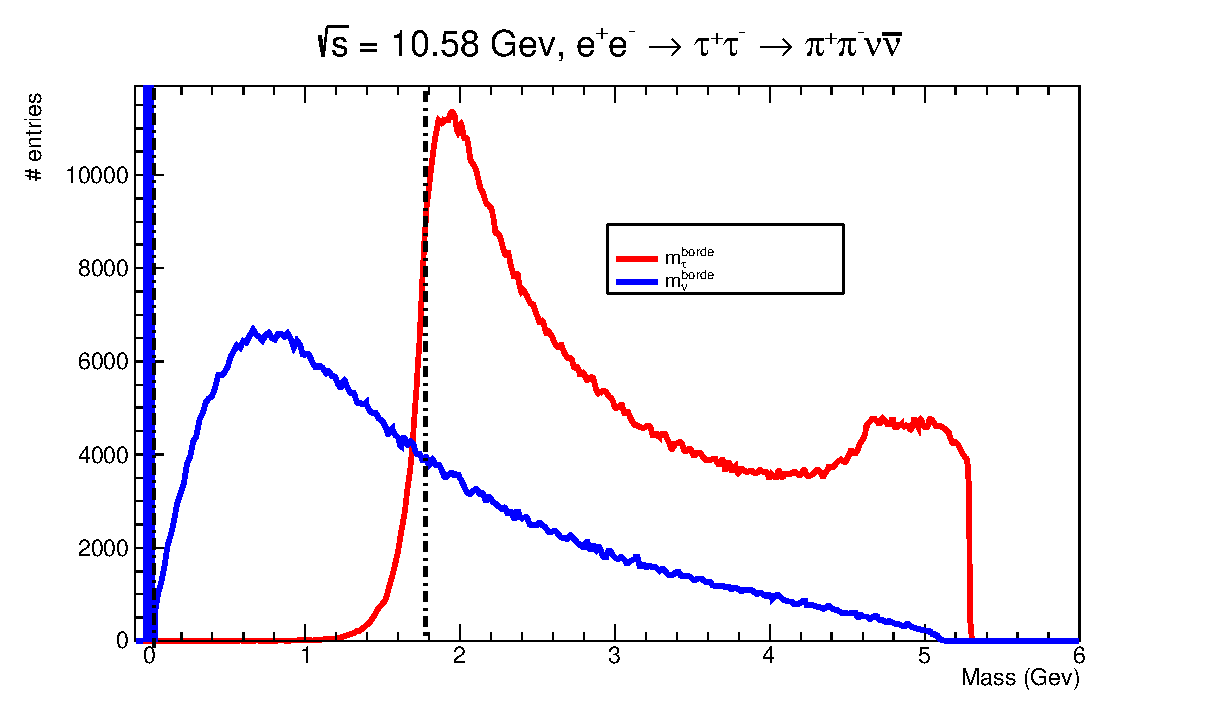
\includegraphics[scale=.6]{Images/m_edge.eps}
    \caption{\small Distribuciones para las variables de ``borde'' (\(m_{\tau}^{borde}\) y \(m_{\nu}^{borde}\)) para \(e^+e^-\rightarrow\tau^+\tau^-\rightarrow\pi^+\pi^-\nu\bar{\nu}\). Las líneas punteadas denotan la masa verdadera \(m_{\tau}\) y \(m_{\nu}\), que para nuestro caso es el valor que se utilizará para la generación (1777.0 MeV).}
    \label{fig:masas}
\end{figure}
\newpage
Tomando las ecuaciones \ref{39} y \ref{41}, una energía CM de 10.5794 \(GeV\)( justo la energía umbral de la resonancia \(\Upsilon(4S)\)), además teniendo encuentra nuestra consideración como límite físico para \(m_X\) de \(\sqrt{s}/2\) y por medio del software ROOT se construyeron las distribuciones (figura \ref{fig:masas}) para el proceso  \(e^+e^-\rightarrow\tau^+\tau^-\rightarrow\pi^+\pi^-\nu\bar{\nu}\).

\subsubsection{Variables ``\texorpdfstring{$M_{min}$}{TEXT}'' y ``\texorpdfstring{$M_{max}$}{TEXT}''}
Para esta parte del proceso, vamos a encontrar un par de variables, reduciendo el potencial del método de estados finales semi-invisibles para el caso en que tanto en señal como en tag tendremos iguales decaimientos 1x1 prong, este proceso es basado en el paper \cite{PhysRevD.102.115001}. 

Usando la ecuación \ref{24} vamos a reproducir otro método para encontrar la masa del leptón tau. Por practicidad, vamos a considerar \(\mu_{1} = \mu_{\nu_{\tau}}\) y \(\mu_{X}=\mu_{\tau}\). Asumiendo \(m_{\nu_{\tau}}=0\), la ecuación \ref{24} se reduce a
\begin{equation}
    A_0(\mu_{\tau}^2)^2+B_0(\mu_{\tau}^2)+D_0\leq0.
\end{equation}
Lo que nos lleva de nuevo a la ecuación \ref{40}, con lo cual
\begin{equation}
    (\mu_{\tau}^2)^2=\pm\frac{\sqrt{B_0^2-4A_0D_0}}{2A_0}-\frac{B_0}{2A_0},
\end{equation}
esto se puede ver como
\begin{equation}
    \left(\mu_{\tau}^{min}\right)^2\leq(\mu_{\tau})^2\leq\left(\mu_{\tau}^{max}\right)^2,
\end{equation}
ya que \(m_{\tau}=\mu_{\tau}\sqrt{s}\), entonces
\begin{equation}
    M_{min}^2\leq m_{\tau}^2 \leq M_{max}^2,
\end{equation}
donde
\begin{eqnarray}
    M_{min}^2&=&\left(\sqrt{s}\right)^2\left(\frac{-B_0-\sqrt{B_0^2-4A_0D_0}}{2A_0}\right),\\
    M_{max}^2&=&\left(\sqrt{s}\right)^2\left(\frac{-B_0+\sqrt{B_0^2-4A_0D_0}}{2A_0}\right).
\end{eqnarray}

Tomando las expresiones anteriores se construyen las distribuciones para las variables \(M_{min}\) y \(M_{max}\) (figura \ref{fig:MminMmaxDistri}), las cuales serán también métodos a probar y que se compararán con el método de ``borde'' para la estimación de la masa del leptón tau.
\begin{figure}[h]
    \centering
    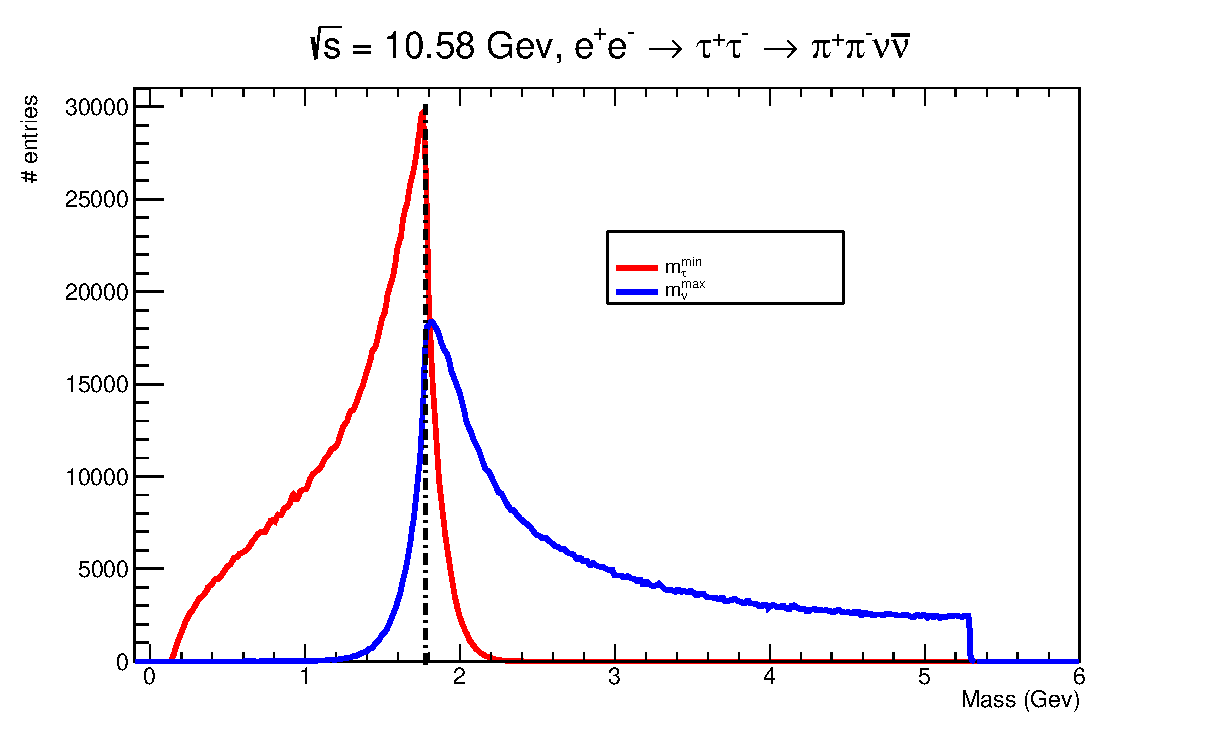
\includegraphics[scale=.6]{Images/m_min_plot.eps}
    \caption{\small{Distribuciones de las variables \(M_{min}\) (rojo) y \(M_{max}\) (azul). La línea punteada es la masa verdadera \(m_{\tau}\).}}
    \label{fig:MminMmaxDistri}
\end{figure}

Como se puede observar en las distribuciones \ref{fig:masas} y \ref{fig:MminMmaxDistri}, la masa que buscamos se relaciona con puntos donde dichas distribuciones tienen una subida pronunciada, son estos puntos los que estimaremos, para esto utilizaremos una función que contiene un parámetro que denominamos estimador.

\subsubsection{Estimador} 
Para ajustar las distribuciones se ha decidido implementar unas funciones de tipo sigmoide, la que mejor se adaptó al ajuste fue la función error complementaria para el caso de la variable \(M_{min}\) y tipo error para las variables \(M_{borde}\) y \(M_{max}\). Por la forma de las distribiciones se decidió multiplicarla por un polinomio para que reproduzca la caída luego de la subida prominente y sumarle un polinomio de segundo orden para ajustar la suave ``cola'' que es común en las tres distribuciones, las funciones de ajuste elegidas son las siguientes
\begin{equation}
    F_1(M_{\tau})=(P_3+P_4M_{\tau}+P_6M_{\tau}^2+P_7M_{\tau}^3)erfc\left(\frac{M_{\tau}-P_1}{P_2}\right)+P_8M_{\tau}^2+P_5M_{\tau}+1, \label{52}
\end{equation}
\begin{equation}
    F_2(M_{\tau})=(P_3+P_4M_{\tau}+P_6M_{\tau}^2+P_7M_{\tau}^3)erf\left(\frac{M_{\tau}-P_1}{P_2}\right)+P_8M_{\tau}^2+P_5M_{\tau}+1, \label{53}
\end{equation}
donde \(P_1\) es el estimador para la masa del leptón tau. Debido a que se busca una función que reproduzca adecuadamente a los datos en una zona de interés, la parametrización es completamente empírica y no un proceso analítico. Por otro lado, el estimador no será exactamente la masa del tau, pero se asumirá que este estará recorrido del valor real, así que se tendrá que corregir el valor del estimador para la función seleccionada en datos simulados, para esto empleamos una muestra oficial de Monte Carlo (MC13a) para la producción de pares de taus, para los cuales sabemos la masa de generación (1777 MeV).

\section{Criterio de selección de datos}
Para la selección de datos se usaron criterios tanto en las trayectorias de las partículas cargadas, como en los fotones, y se utilizaron los siguientes parámetros
\begin{table}[h!]
\centering
 \begin{tabular}{||c | c||} 
 \hline
 Criterio de trayectorias & Criterio para fotones  \\ [0.5ex] 
 \hline\hline
 \(p_t\)>0.1(GeV) & E> 0.2 (GeV)\\ 
 \hline
 -0.8660< cosTheta< 0.9563 & -0.8660< cosTheta< 0.9563  \\
 \hline
 -3.0< dz< 3.0 & clusterNHits> 1.5  \\
 \hline
 dr< 1.0 & 0.115 < M < 0.152  \\
 \hline
 \end{tabular}
 \caption{\small{Criterio de selección para las trayectorias de partículas cargadas y para fotones}}\label{table:crite}
\end{table}

De la tabla \ref{table:crite}, \(p_t\) es el el momento transversal de la partícula cargada, E sería la energía del fotón, \(cosTheta\) es el coseno del ángulo que comprende el detector (aceptancia del detector), \(dz\) es la distancia de la reconstrucción de la trayectoria respecto al IP sobre el eje z, \(dr\) es la distancia de la misma en la coordenada radial. Ambos valores, \(dz\) y \(dr\) están expresados en \(cm\). Por otro lado, el parámetro \(clusterNHits\) hace referencia el número de cristales activados en el ECL para reconstruir un fotón. 0.115 < M < 0.152 es el criterio para la reconstrucción de \(\pi^0\)'s. 

La selección de eventos requirió que se hiciera un filtrado haciendo algunos cortes en ciertas variables, para ello se utilizaron los siguientes \begin{table}[h!]
\centering
 \begin{tabular}{||c||} 
 \hline
 Criterio de selección de eventos \\ [0.5ex] 
 \hline\hline
 nGoodTracks = 2 \\ 
 \hline
 Thrust<0.99 \\
 \hline
 0<EoverP<0.8 \\
 \hline
 N(\(\pi^0\))=0\\
 \hline
 N(\(\gamma\))\leq1\\
 \hline
 \end{tabular}
 \caption{\small{Criterio de selección de eventos}}\label{table:crite}
\end{table}

\(nGoodTracks\) es el número de buenas partículas cargadas, para nuestro caso usamos dos, y así reproducir la topología que nos interesa. \(Thrust\) es una variable que se define por medio del vector unitario \(\hat{u}_{thrust}\) perpendicular a la línea que separa la señal y  (figura \ref{fig:MminTopo}), el valor del \(Thrust\) se define como \(V_{thrust}\equiv\sum_{i}\frac{|\mathbf{p}_i^{cm} \cdot \hat{n}_{thrust}|}{\sum_{i}|\mathbf{p}_{j}^{cm}|}\), de manera que dicho valor sea el máximo,  Con el vector \(\hat{n}_{thrust}\) y el valor del thrust se separan los decaimientos en dos hemisferios. La variable EoverP que es la razón entre la energía depositada en el calorímetro y el momento de partículas cargadas, se exige 0<\(EoverP\)<0.8 para garantizar una mayor cantidad de piones presentes en los tracks (esta variable se usó en el proceso de reconstrucción en la variable \(pionIDcuts\)). \(N(\pi^0)\) es el número de piones neutros y \(N(\gamma)\) es el número de fotones.
\begin{figure}[h]
    \centering
    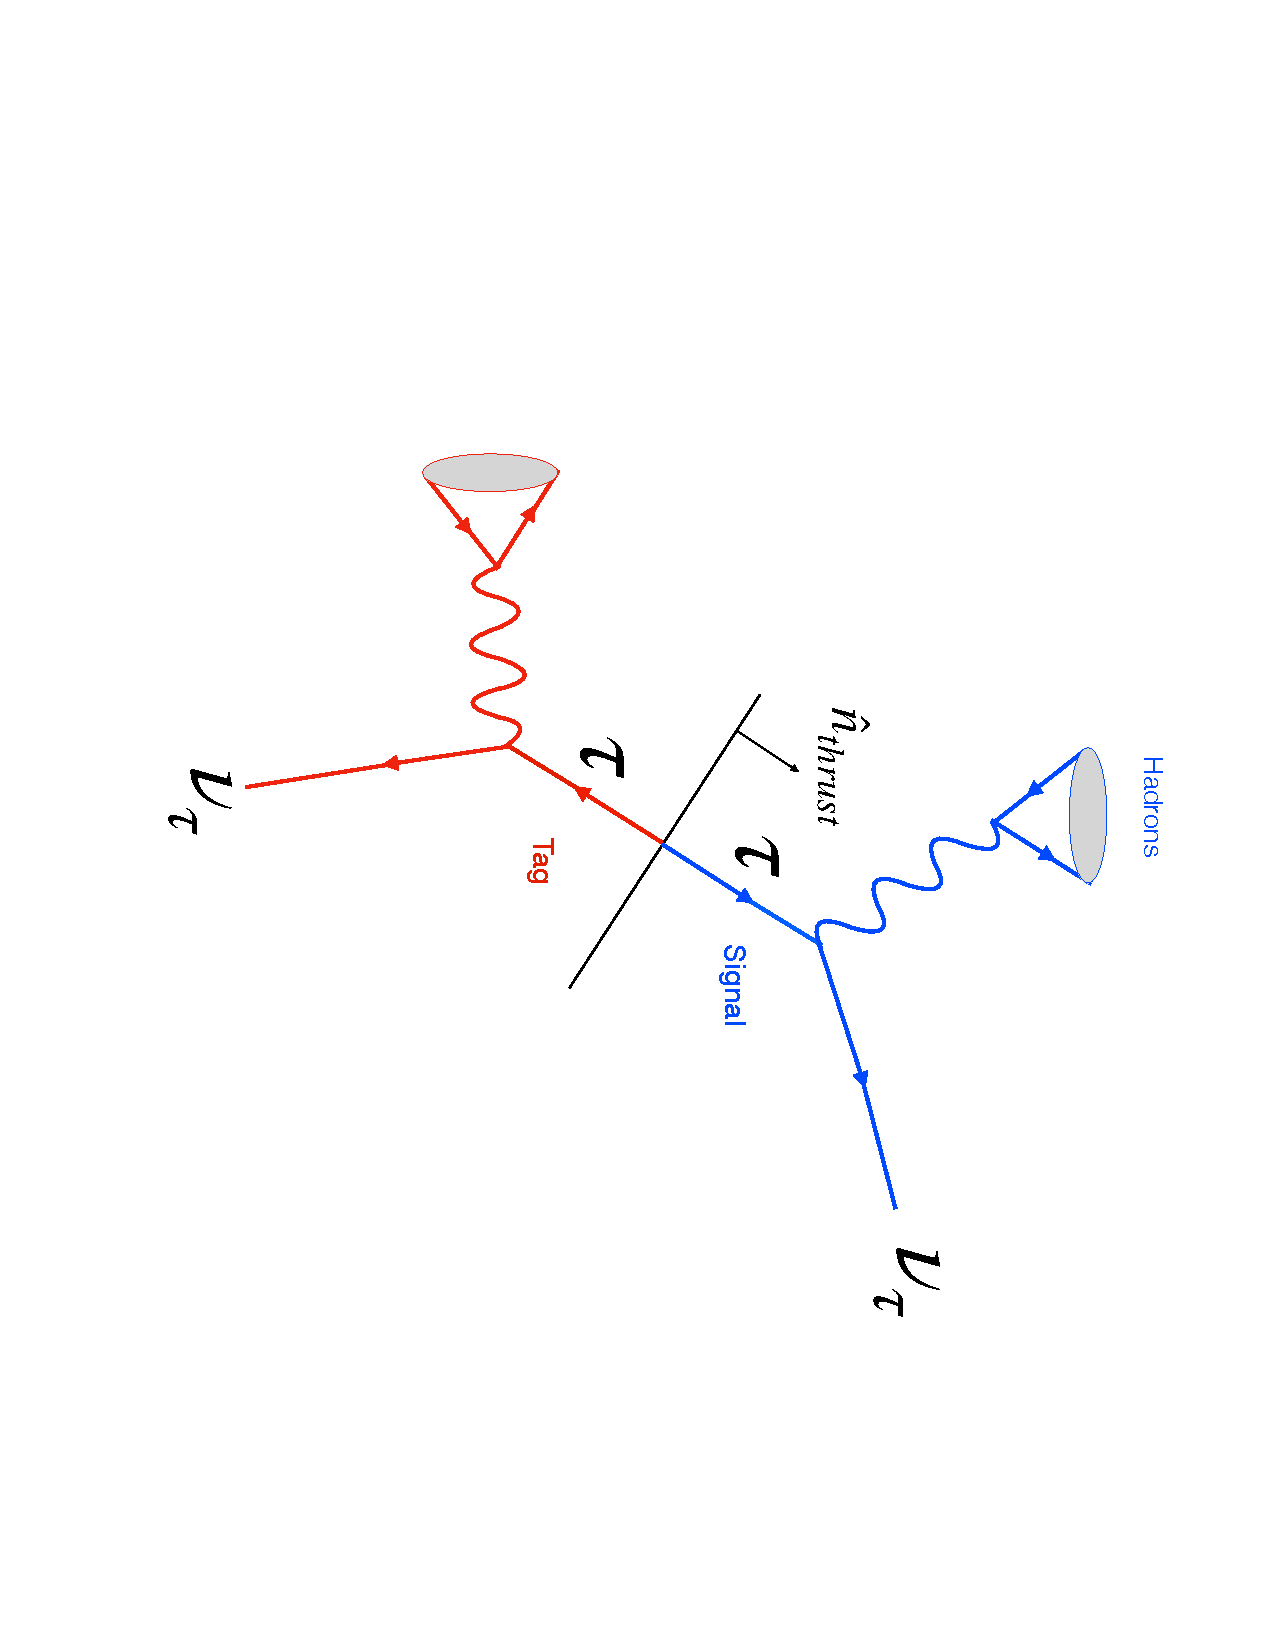
\includegraphics[scale=.05]{Images/Diagram1x1.jpg}
    \caption{\small{Esquema señal-tag en topología 1x1 prong en decaimiento del tau. Se muestra la dirección del vector \(\hat{n}_{thrust}\) que separa la señal del tag.}}
    \label{fig:MminTopo}
\end{figure}

Con los requerimientos anteriores, tanto de trayectorias, como en fotones y en selección de eventos se reconstruyeron los pares de taus que cumplen dichos requisitos, decayendo tanto tag como señal en 1-prong, para nuestro caso, en un pión cargado y un neutrino del tau. Con esta información se logra hacer la reconstrucción del par de taus (taupair).

\section{Database}

Se utilizaron como datos, los generados mediante método Monte Carlo en la campaña oficial de Belle II MC13a. Los datos fueron tratados como si provinieran directamente del detector, es decir, sobre ellos se aplicaron los cortes de selección de eventos, a esto se le conoce como ``skim''. La muestra de MC usada es equivalente a una luminosidad de 100 \(fb^{-1}\) (Cantidad de datos equiparable con los datos que hasta hace poco se habían recolectado en Belle II, cifra superada en junio del 2021, hasta el momento se han recolectado 200 \(fb^{-1}\)), las muestras de MC usadas se pueden separar en dos, Generic (Genérica) y Lowmulti (Baja multiplicidad) como se observa en la tabla \ref{table:skim}. En la versión release-04-00-03 del software basf2 se reconstruyó el decaimiento de interés, usando Tauola que proporciona todos los posibles decaimientos del leptón tau. Las muestras se generan en la colaboración para una masa de 1777 \(MeV\), siendo para este estudio considerada la masa verdadera.
\begin{table}[h!]
\centering
 \begin{tabular}{|| p{3cm} | p{3cm} | p{3.5cm} ||} 
 \hline
 Etiqueta de producción & Tipo de evento & Luminosidad \\ [0.5ex] 
 \hline\hline
 MC13a  & mixed & 100 \(fb^{-1}\), \\
 (Generic)& &\\
 & charged &\\
 & & correspondiente a\\
 & uubar & mixed: 51 M\\
 & & charged: 54 M\\
 & ddbar & uubar: 160.5 M\\ 
 & & ddbar: 40.1 M\\
 & ccbar & ssbar: 38.3 M\\
 & & ccbar: 132.9 M\\
 & ssbar & taupair: 91.9 M\\
 & &\\
 & taupair &\\
 \hline
 MC13a  & eeee & 100 \(fb^{-1}\) \\
 (Lowmulti)& &\\
 & mumu &\\
 & & \\
 & eemumu &\\
 &\hline&\hline \\
 & ee & 10 \(fb^{-1}\)\\
 \hline
 \end{tabular}
 \caption{\small{Muestras de la campaña MC13a, Generic y Lowmulti con su correspondiente luminosidad}}\label{table:skim}
\end{table}
 Tendremos como señal el proceso de decaimiento \(\tau\rightarrow\pi\nu_{\tau}\), este se encuentra dentro de la muestra "taupair", dicha muestra se filtró inicialmente con los cortes de selección, luego con los criterios de selección de eventos y por último usando la variabe ``\(MCMode\)'', esta permite seleccionar el decaimiento que nos compete con un indicador como se muestra en la figura \ref{fig:TauDecay} , donde el modo de decaimiento 1x1-prong usado es el número 3. Ya seleccionando la señal se creó el histograma de la distribución para cada una de las variables que se estudiaron.
\begin{figure}[h]
    \centering
    \includegraphics[scale=.8]{Images/TauDecays.png}
    \caption{\small{Marcadores para los distintos decaimientos del tau presentes en TauolaBelle, la variable de identificación de estos canales es denominada \textit{MCMode}}}.
    \label{fig:TauDecay}
\end{figure}

\subsection{Estimador para \texorpdfstring{$M_{borde}$}{TEXT}}
Los demás procesos que no sean el decaimiento que denominamos como señal son considerados como ruido. Para este trabajo se consideran procesos de baja multiplicidad (\(ee,ee\mu\mu,\mu\mu,eeee\)), \(q\bar{q}\) (\(q = u,d,s,c\)), \(B\bar{B}\) y todos los procesos posibles en decaimientos del leptón tau (figura \ref{fig:TauDecay}), de estos últimos se hace la distinción entre señal y ruido. La señal es el proceso \(\tau\rightarrow\pi\nu\), los demás decaimientos del tau serán considerados como ruido y la denominaremos como ``\(\tau\)BG''. Al agregar todas las muestras anteriores a una sola distribución se reproduce la distribución que se obtendría con datos reales de Belle II. Para obtener la señal se debe separar señal de ruido, para esto se decide usar un método de Maching Learning, como lo son los BDT (\textit{Boosting Decision Trees}), implementado en ROOT por medio de un ambiente para el procesamiento y evaluación de clasificación multivariada como lo es TMVA (\textit{Toolkit for Multivariate Data Analysis}) \cite{Hocker:2007ht}.

\subsubsection{BDT}

Por medio de TMVA y usando catorce variables cinemáticas de evento y dos de identificación de partículas se hizo el entrenamiento para el BDT. Las variables usadas fueron las siguientes.


\begin{itemize}
    \item \textit{track1\_cosToThrustOfEvent}:  coseno del ángulo entre la partícula cargada y el eje de thrust del evento.
    \item 
    \textit{track1\_clusterE}: energía del clúster ECL corregida por fugas y ruido.
    \item 
    \textit{visibleEnergyOfEventCMS}: energía visible en el marco de referencia CM.
    \item
    \textit{missingMomentumOfEventCMS}: magnitud del momento perdido en el marco de referencia CM
    \item
    \textit{missingMomentumOfEventCMS\_theta}: ángulo \(\theta\) del momento perdido en el CM
    \item
    \textit{missingMass2OfEven}: masa perdida al cuadrado
    \item
    \textit{track1\_EoverP}: EoverP de la partícula cargada del track 1
    \item
    \textit{track1\_pt}: momento total del track 1
    \item
    \textit{track1\_pionID}: pionID para el track 1
\end{itemize}

Así como las variables correspondientes a la otra partícula cargada del decaimiento que se denomina ``track2''.

Uno de los resultados del BDT fue que las variables que más separación entre ruido y señal aportaron fueron las de \(pionID\). El TMVA crea las distribuciones de clasificación (figura \ref{fig:bdtFom}), con ayuda de dicha distribución se debe seleccionar el mejor corte en esta variable nueva (BDT), y así garantizar una eficiencia óptima en la separación ruido-señal, para encontrar el mejor valor de BDT se usó la figura de mérito
\begin{equation}
    FOM=2\left(\sqrt{N_{sig}+N_{bkg}}-\sqrt{N_{bkg}}\right)\label{fom},
\end{equation}
obteniéndose un valor para el BDT de alrededor de 0.2, nótese que dicho valor es el punto donde la FOM tiene un máximo. Se elige para el método \(m^{borde}_{\tau}\) un valor del BDT de 0.2. Las muestras se han dividido en tres partes. La primera para realizar el entrenamiento del TMVA y crear los BDT's, la segunda será para encontrar el estimador y el sesgo de los diferentes métodos y la tercera se usará como ``datos reales'' para el análisis final y estimación de la masa del leptón tau en cada método.
\begin{figure}%
    \centering
    \subfloat[\centering  ]{{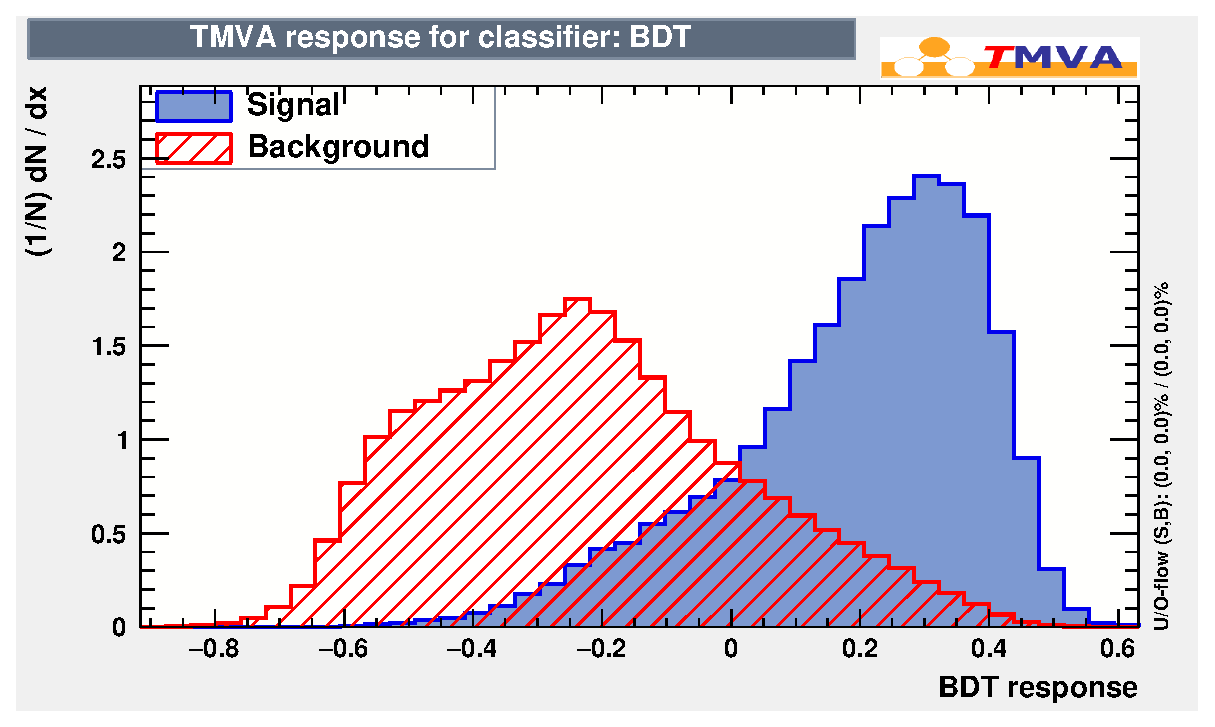
\includegraphics[width=7.5cm]{Images/bdt_bg_sig.eps} }}%
    \qquad
    \subfloat[\centering  ]{{\includegraphics[width=7.5cm]{Images/FOM.png} }}%
    \caption{(a) Distribución de respuesta del BDT y clasificada como señal y ruido. (b) FOM}
    \label{fig:bdtFom}%
\end{figure}
Inicialmente, se grafica la distribución de la variable \(m^{borde}_{\tau}\) sólo para señal y se muestra la distibución completa y un zoom en la región de ajuste en la figura \ref{fig:mEdgeDistri}, esto con propósito de tener bien definida la señal y para realizar el ajuste más óptimo. 

De la figura \ref{fig:ajusteMedge}, en la región de ajuste se observan dos grandes componentes, una es la principal que se refiere a la señal y la otra es el ruido de fondo \(\tau\)BG. Lo anterior luego de hacer el corte en BDT, se deben ajustar ambas componentes y unirlas en una sola para encontrar el estimador para la masa del leptón tau. Se elije usar para la componente de \(\tau\)BG una función de ajuste o función de distribución de probabilidad (PDF) de tipo lineal de la forma
\begin{equation}
    F_3(M_{\tau})=A_1+A_2M_{\tau}, \label{55}
\end{equation}
con la ayuda de la PDF \ref{53} se ajustó la señal y el ruido se ajustó con \ref{55}, luego se debían unir ambos ajustes, es decir ``sumar'' las PDF's, para ello se usó una suma paramétrica de la forma
\begin{equation}
    F_{4}=fS_{PDF}+(1-f)B_{PDF},
\end{equation}
donde \(S_{PDF}\) es la PDF para la señal, \(B_{PDF}\) la PDF para el ruido y \(f\) es un coeficiente menor que 1, es decir, es una constante sujeta a las condiciones de normalización.


Para una muestra de pares tau se realizó la medición de la masa y se compara el estimador con el valor de la masa de generación \(m_{\tau}=1777.00\) MeV. Para el caso de la variable \(M_{borde}\) en la región de ajuste y utilizando la adición de PDF's se obtuvo un valor para el estimador \(P1=1765.80\pm6.0\) MeV (figura \ref{fig:ajusteMedge} (a)), la diferencia en la masa es de \(\Delta_{m}=11.2\) MeV. Con este valor de bias se corrige el valor obtenido con la muestra restante, la de datos reales (figura \ref{fig:ajusteMedge} (b)), corregimos la estimación de la masa para los datos reales, obtenemos un valor para la masa del tau de \(m_{\tau} = 1772.40\pm 7.38\) MeV. Para el valor final en las incertidumbres se decidió combinarla y para ello se usó la suma en cuadraturas. 

\begin{figure}[h]
  %\setcapwidth{0.6\textwidth}
  \checkoddpage
  \edef\side{\ifoddpage r\else l\fi}%
  \makebox[\textwidth][\side]{%
    \begin{minipage}[t]{0.58\textwidth}
      \centering
    \subfloat[\centering  ]{{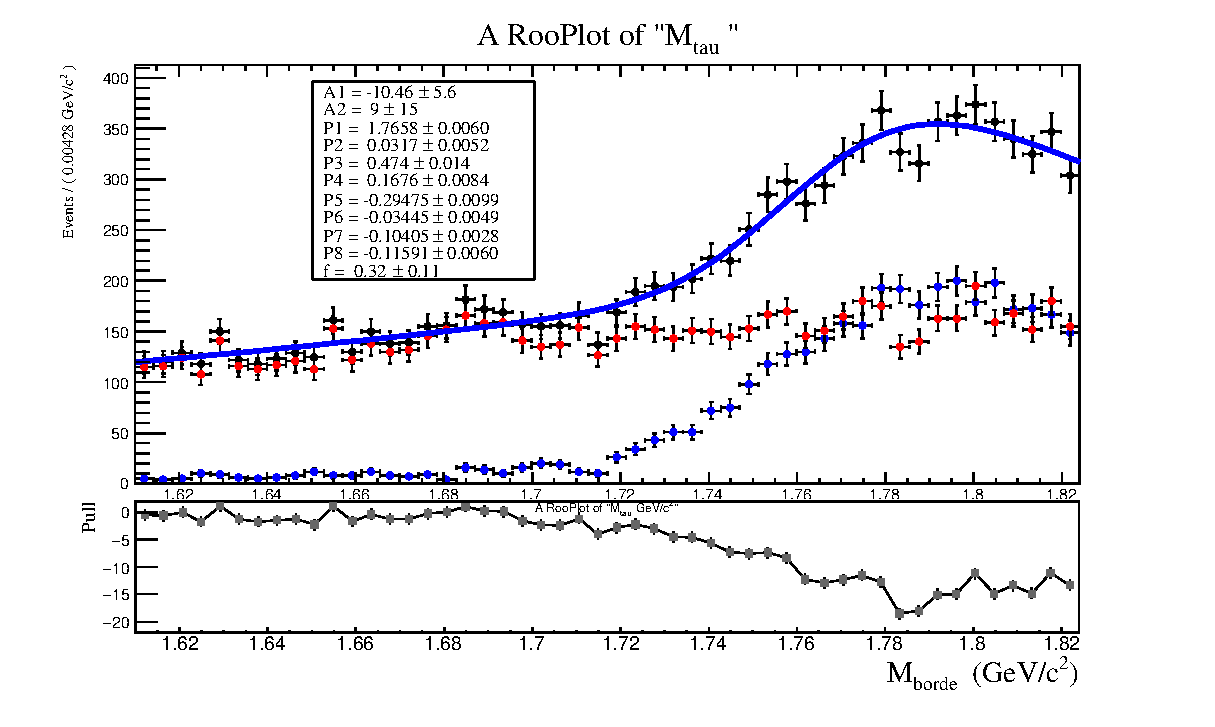
\includegraphics[width=\textwidth]{Images/m_borde_bkg_sig.eps} }}
      %\caption{Caption 1}
    \end{minipage}%
    \hfill
    \begin{minipage}[t]{0.58\textwidth}
      \centering
    \subfloat[\centering  ]{{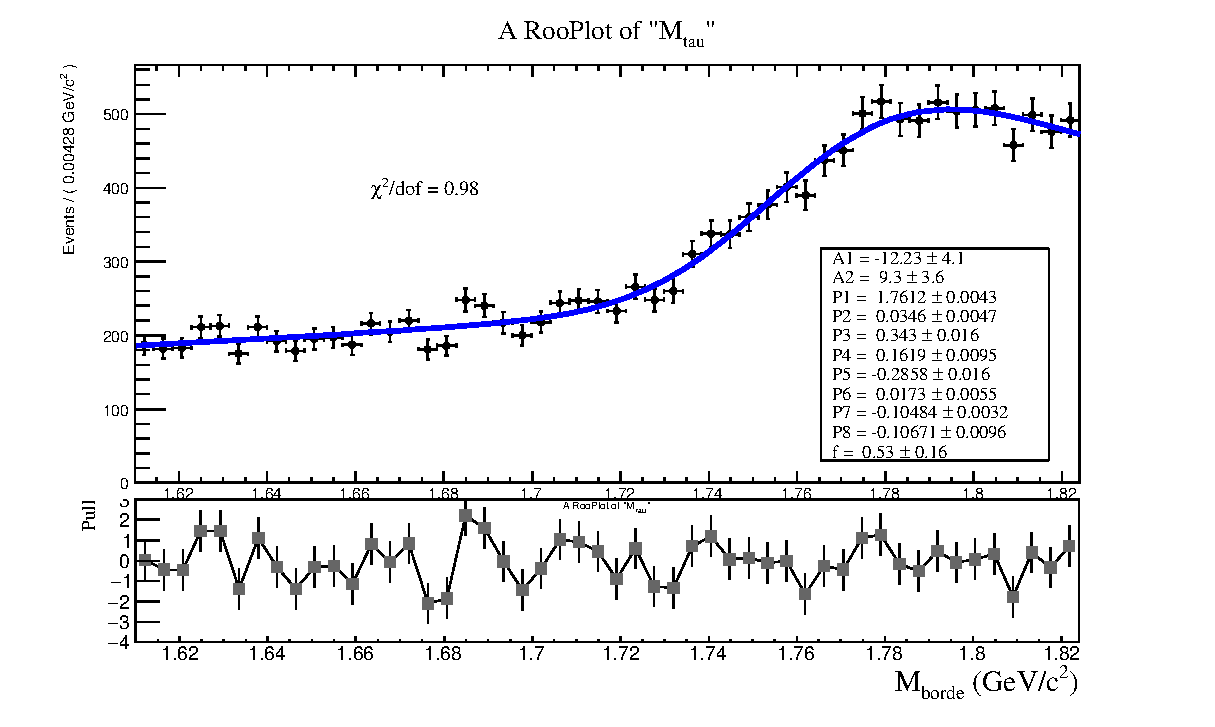
\includegraphics[width=\textwidth]{Images/m_borde_real.eps} }}
      %\caption{Caption 2}
    \end{minipage}%
  }%
  \caption{\small{(a) Ajuste \(M_{borde}\) para ruido y señal. En rojo \(\tau BG\), en azul \(\tau \rightarrow \pi\nu \) y en negro la suma de señal más ruido. Valor para el estimador de la masa de \(1765.8\pm5.2\) MeV.  (b) Ajuste de la distribución de la variable \(M_{borde}\) para datos ``reales'' con un valor para el estimador de la masa de \(1761.2\pm4.3\) MeV.}}
  \label{fig:ajusteMedge}
\end{figure}

\newpage
\subsection{Estimador para \texorpdfstring{$M_{min}$}{TEXT}}



Para el caso de la variable \(M_{min}\) se muestra la distribución completa de sólo señal y en la región de ajuste en la figura \ref{fig:mMinDistri}. Usando el corte BDT>0.2, se separa en esta variable señal de ruido de una forma más prolija, las contribuciones de ruido se pueden ver en las figuras del apéndice B. En la zona de ajuste se observa que el ruido \(\tau BG\) contribuye menos que en el caso anterior, pero se decide de igual forma usar la PDF para el ruido (\ref{55}) y para la señal la función error complementaria (\ref{52}), gráficamente este proceso se puede ver en la figura \ref{fig:ajusteMmin} (a).

Se obtiene un valor para el estimador de \(P1=1777.70\pm 0.16\) MeV, una diferencia respecto al valor real de \(\Delta_{m}=-0.70\) MeV. Ya considerando la muestra real (figura \ref{fig:ajusteMmin} (b)) y con el valor de la diferencia corregimos la estimación de la masa y en datos reales  se obtiene un valor para la masa del leptón tau de \(m_{\tau} = 1777.06 \pm 0.47\) MeV.
\begin{figure}[h]
  %\setcapwidth{0.6\textwidth}
  \checkoddpage
  \edef\side{\ifoddpage l\else r\fi}%
  \makebox[\textwidth][\side]{%
    \begin{minipage}[t]{0.57\textwidth}
      \centering
    \subfloat[\centering  ]{{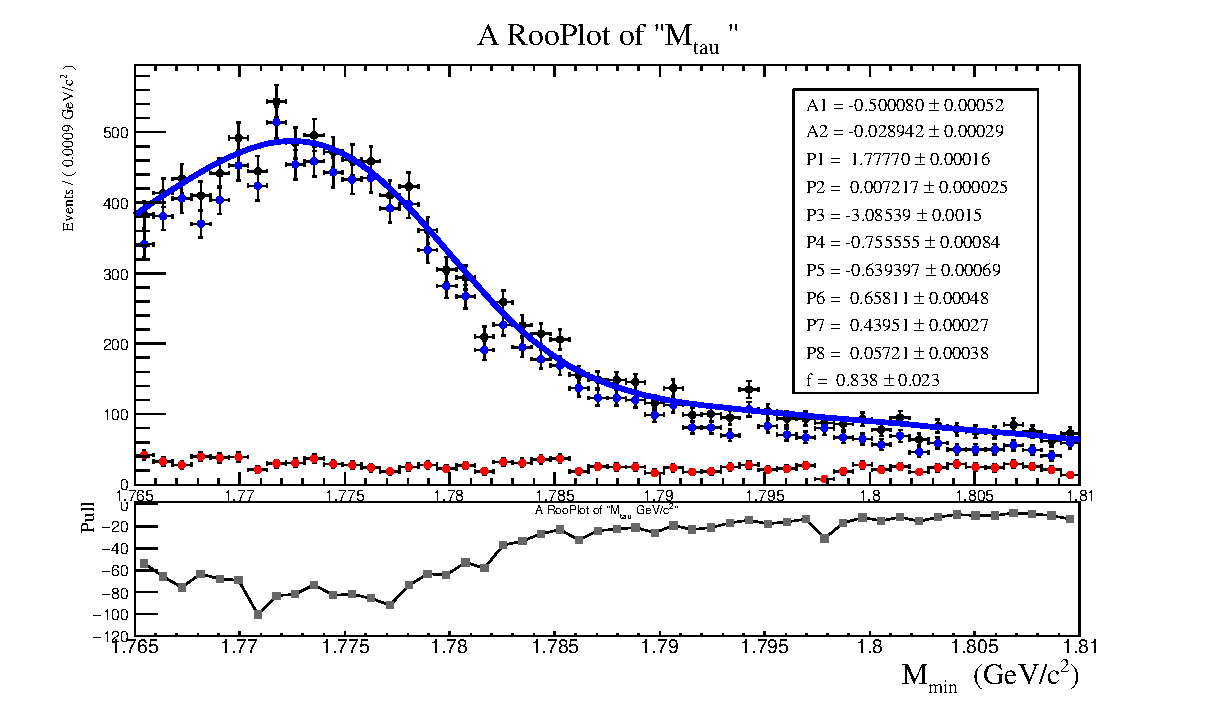
\includegraphics[width=\textwidth]{Images/m_min_bkg_sig.eps} }}
      %\caption{Caption 1}
    \end{minipage}%
    \hfill
    \begin{minipage}[t]{0.57\textwidth}
      \centering
    \subfloat[\centering  ]{{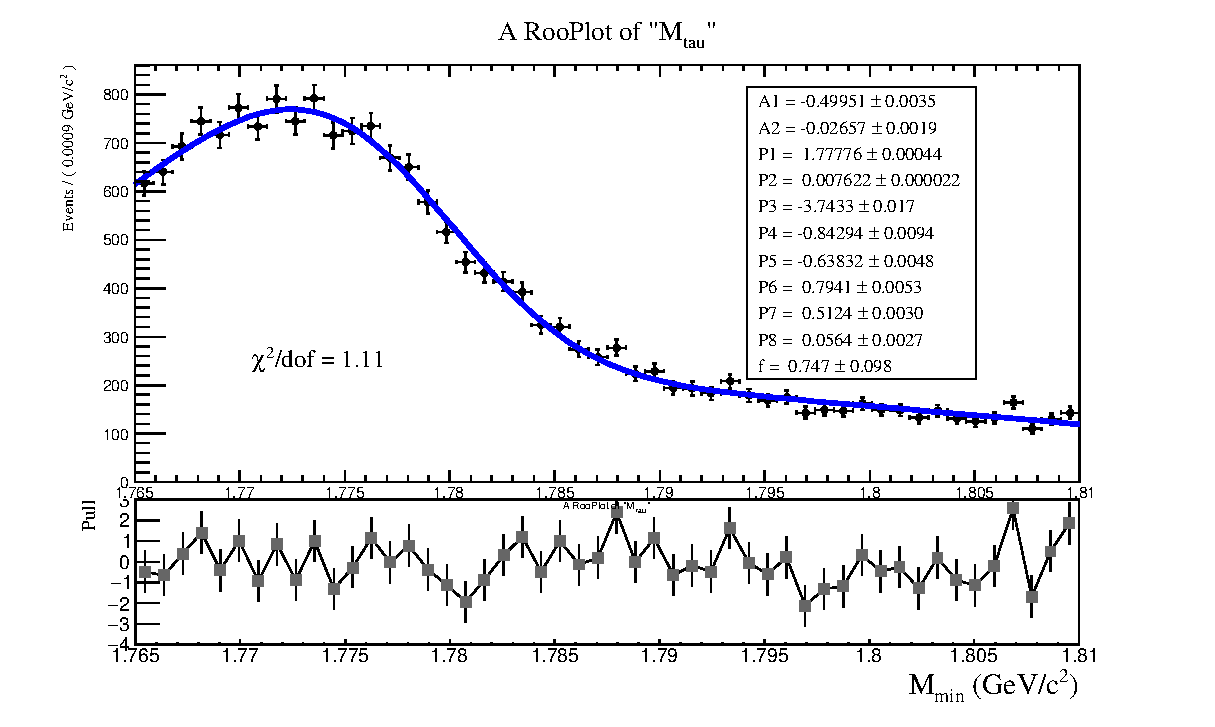
\includegraphics[width=\textwidth]{Images/m_min_real.eps} }}
      %\caption{Caption 2}
    \end{minipage}%
  }%
  \caption{\small{(a) Ajuste de \(M_{min}\) para ruido y señal. En rojo \(\tau BG\), en azul, \(\tau \rightarrow \pi\nu \) y en negro la suma de señal más ruido. Valor para el estimador de la masa de \(1777.70\pm0.16\) MeV.  (b) Ajuste de la distribución \(M_{min}\) en datos reales con un valor para el estimador de la masa de \(1777.76\pm0.44\) MeV.}}
  \label{fig:ajusteMmin}
\end{figure}


\newpage
\subsection{Estimador para \texorpdfstring{$M_{max}$}{TEXT}}

Siguiendo el mismo proceso para el último método, la variable \(M_{max}\) sólo considerando señal, se muestra la distribución completa junto con el zoom en la región de ajuste en el apéndice C. En este caso se logra obtener un valor para el estimador de masa de \(P1=1775.16\pm0.14\) MeV (figura \ref{fig:ajusteMmax} (a)) para una diferencia en la masa de \(\Delta_{m}=1.84\) MeV. Corrigiendo entonces con este bias al valor obtenido en el ajuste a los datos reales se obtiene un valor para la masa de \(m_{\tau}=1781.44\pm0.38\) MeV.
\begin{figure}[h]
  %\setcapwidth{0.6\textwidth}
  \checkoddpage
  \edef\side{\ifoddpage r\else l\fi}%
  \makebox[\textwidth][\side]{%
    \begin{minipage}[t]{0.57\textwidth}
      \centering
    \subfloat[\centering  ]{{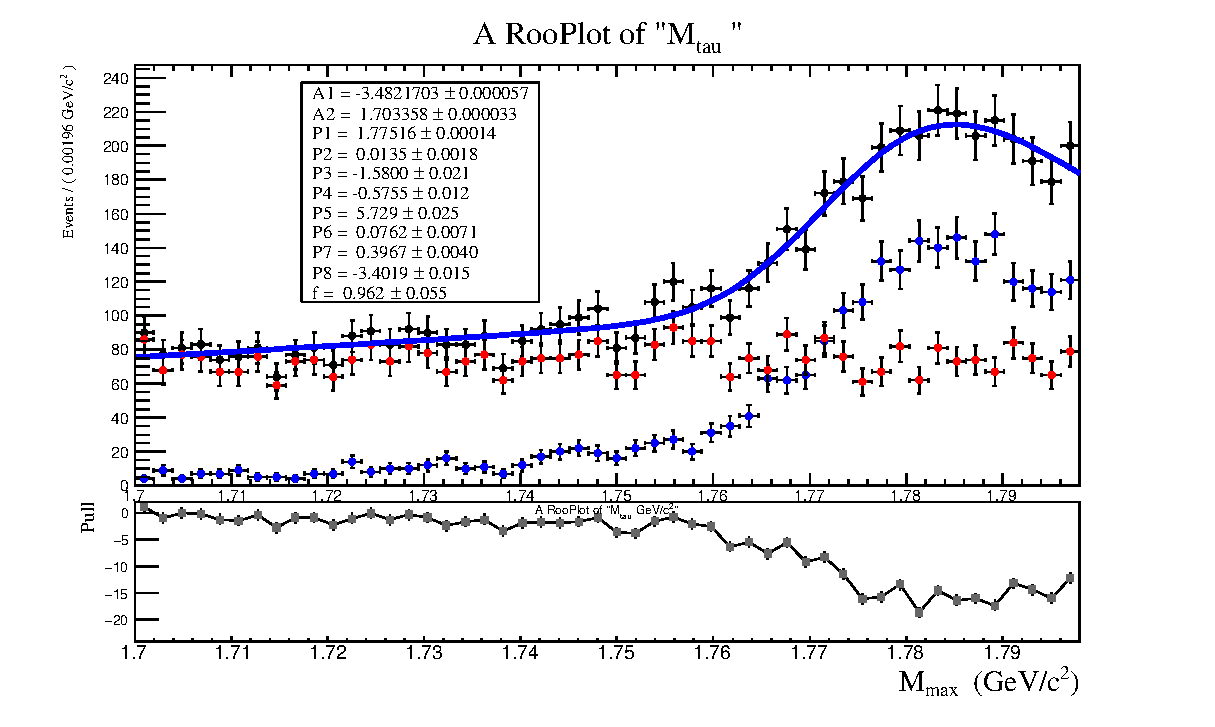
\includegraphics[width=\textwidth]{Images/m_max_bkg_sig.eps} }}
      %\caption{Caption 1}
    \end{minipage}%
    \hfill
    \begin{minipage}[t]{0.57\textwidth}
      \centering
    \subfloat[\centering  ]{{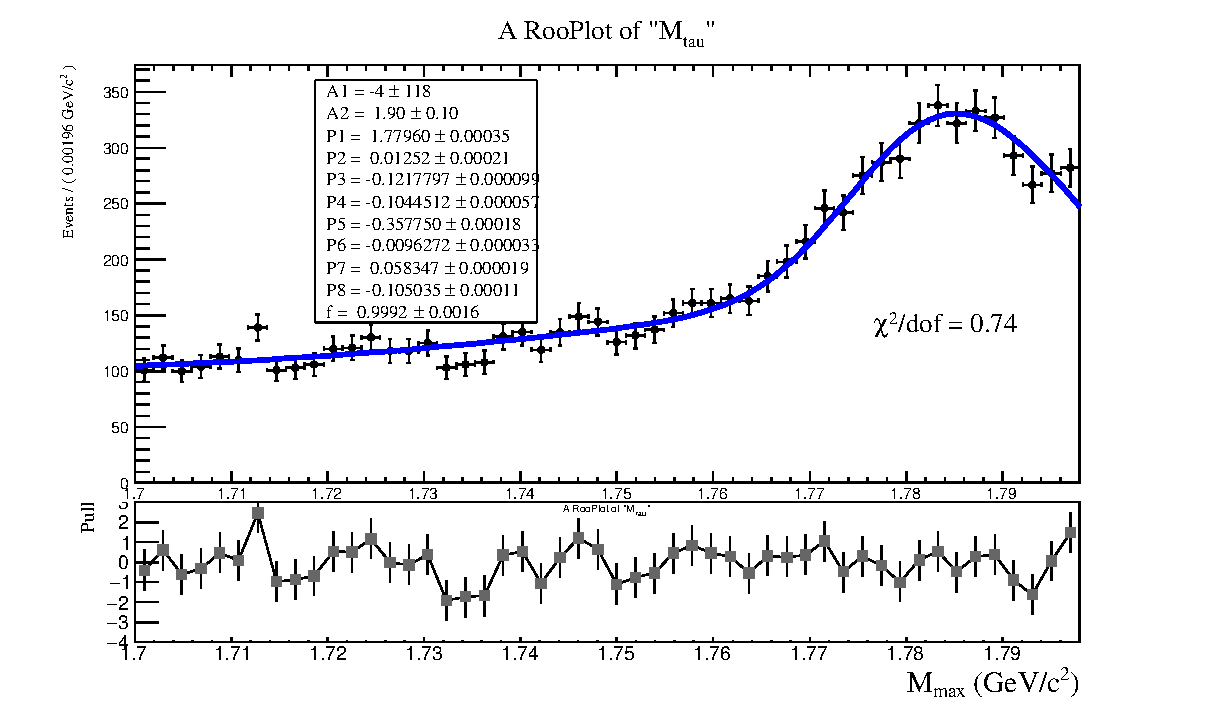
\includegraphics[width=\textwidth]{Images/m_max_real.eps} }}
      %\caption{Caption 2}
    \end{minipage}%
  }%
  \caption{\small{(a) Ajuste de \(M_{max}\) para ruido y señal. En rojo \(\tau BG\), en azul, \(\tau \rightarrow \pi\nu \) y en negro la suma de señal más ruido. Valor para el estimador de la masa de \(1775.16\pm0.14\) MeV.  (b) Ajuste de la distribución de \(M_{max}\) en datos reales con un valor para el estimador de \(1779.60\pm0.35\) MeV.}}
  \label{fig:ajusteMmax}
\end{figure}

\chapter{Posibles fuentes de errores sistemáticos}
En el momento en que una medición como la realizada en la presente tesis se aplica a datos producidos por el experimento se deben considerar errores que van más allá de las incertidumbres estadísticas. No hay una única manera de calcular las incertidumbres sistemáticas en un experimento, pero la experiencia recavada por investigadores y la repetición de ciertas medidas a lo largo de tiempo ha proporcionado que se logren identificar fuentes principales de este tipo de errores, como lo son, diseño del experimento, teniendo en cuenta los propios componentes del mismo, la eficiencia, la calibración y resolución.

También es importante resaltar que la manera en cómo se lleva a cabo el proceso de medición ocasiona la aparición de incertidumbres sistemáticas, como en nuestro caso, vemos que todos los métodos basados en un ``edge'' o ``borde'' como lo llamamos en este trabajo tienen intrínsecamente un sesgo. Otras posibles fuentes de sistemáticos pueden ser los modelos teóricos, los ruidos, simulación MC y hasta el investigador mismo.

Para en nuestro caso podemos tener las siguientes posibles fuentes adicionales de incertidumbres sistemáticas

\begin{itemize}
    \item \textbf{Sistemático debido a la elección de la función de ajuste}.\\
    Considerando la arbitrariedad en la elección de la PDF para ajustar a los datos es necesario analizar la variación en la medición de la masa usando diferentes funciones de ajuste, para este caso se debe calcular la varianza de las diferentes masas halladas, el resultado de esto se asocia con el sistemático
    \item \textbf{Sistemático debido al rango del ajuste}.\\
    Cuando  se escogen diferentes rangos de ajuste, el valor del estimador cambiará, esto hace que se deba considerar una incertidumbre respecto a la medición de la masa.
    \item \textbf{Sistemático asociado a la incertidumbre en la energía del haz}. \\
    Desde la reconstrucción completa de mesones B, teniendo en cuenta la incertidumbre en la masa del B, la calibración en la reconstrucción de las trayectorias y el efecto del ancho en la resonancia \(\Upsilon(4S)\) se calcula la energía del haz. Viendo cómo se propaga el error del anterior cálculo en los datos de MC se puede lograr hallar el sistemático debido a la energía del haz.
    \item \textbf{Sistemático asociado a productos del decaimiento del \(\tau\) mal identificados y eventos no-\(\tau^+\tau^-\)}.\\
    Se debe buscar estructura en la región de ajuste  que pueda afectar la medición de la masa del tau.   
    
\end{itemize}
\chapter{Conclusiones}
\begin{itemize}
    \item En este trabajo se adaptaron tres métodos para la medición de la masa del leptón tau basados en la solucionabilidad de ecuaciones cinemáticas. El primero de ellos para una región completa de solución que denominamos ``\(M_{borde}\)'', en este se observó que la densidad de eventos tiende a ser mayor cerca al punto de masa verdadera. Los otros dos métodos ``\(M_{min}\)'' y ``\(M_{max}\)'' tuvieron como aproximación la consideración de masa nula para el neutrino del tau. Como resultado principal de esta tesis se optine que el mejor método para la medición de la masa del leptón tau en la topología \textit{1x1-prong} (que aún no ha sido implementada en la colaboración Belle II) es el método ``\(M_{min}\)'', donde se obtiene un valor para la masa del leptón tau de \(m_{\tau}=1777.06\pm0.47\) MeV. Este resultado se obtiene con los datos oficiales de Belle II simulados en la campaña MC13a.
    \item Los métodos para realizar mediciones de masa en decaimientos cuyos productos finales se clasifican como semi-invisibles usados en esta tesis naturalmente poseen un sesgo debido a la imposibilidad de reconstruir en su totalidad dichos decaimientos. El método que presentó un mayor sesgo fue ``\(M_{borde}\)'' con un valor de \(\Delta_{m}=11.2.\) MeV.
\end{itemize}

\begin{appendices}
  \chapter{Gráficos referentes a la variable \texorpdfstring{$M_{borde}$}{TEXT}}
\begin{figure}[h]
  %\setcapwidth{0.6\textwidth}
  \checkoddpage
  \edef\side{\ifoddpage r\else l\fi}%
  \makebox[\textwidth][\side]{%
    \begin{minipage}[t]{0.56\textwidth}
      \centering
    \subfloat[\centering  ]{{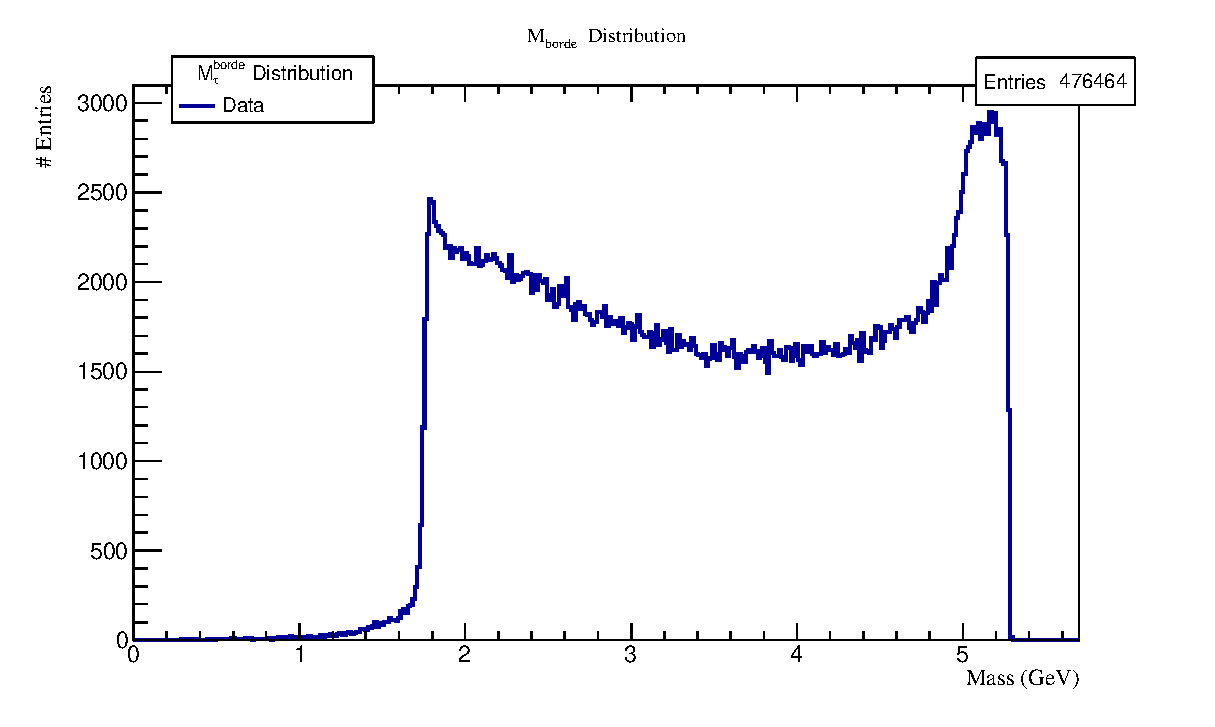
\includegraphics[width=\textwidth]{Images/m_edge_distri.eps} }}
      %\caption{Caption 1}
    \end{minipage}%
    \hfill
    \begin{minipage}[t]{0.56\textwidth}
      \centering
    \subfloat[\centering  ]{{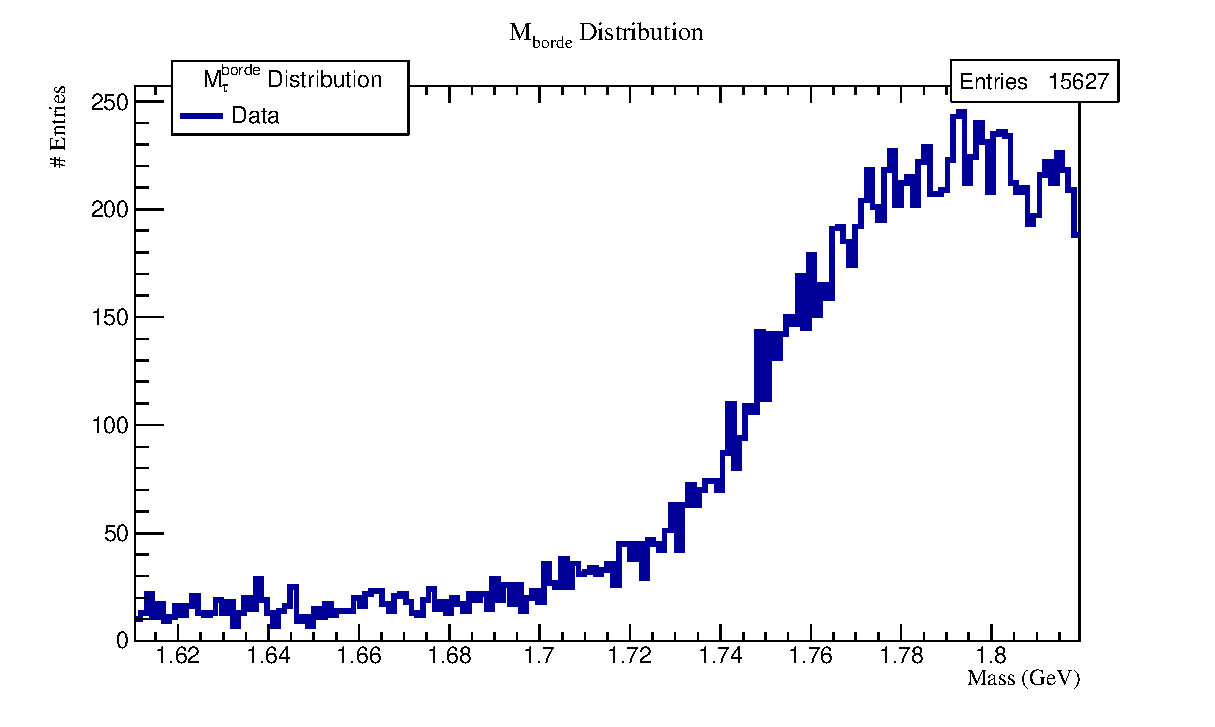
\includegraphics[width=\textwidth]{Images/m_edge_fit_distri.eps} }}
      %\caption{Caption 2}
    \end{minipage}%
  }%
  \caption{\small{(a) Distribución completa de la variable \(m^{borde}_{\tau}\) (sólo señal) de la muestra ``taupair'' de MC13a del experimento Belle II. (b) Distribución de la variable \(m^{borde}_{\tau}\) en la región de ajuste.}}
  \label{fig:mEdgeDistri}
\end{figure}
\begin{figure}[h]
    \centering
    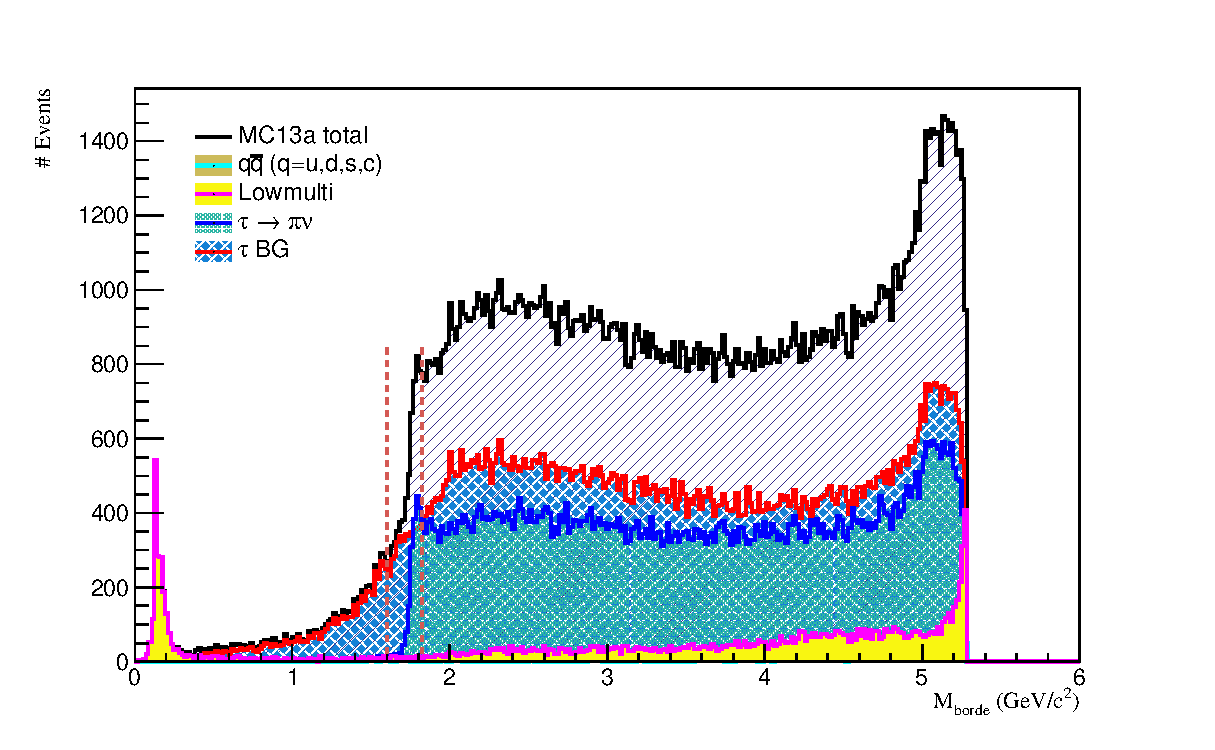
\includegraphics[scale=.6]{Images/m_edge_bdt_all.eps}
    \caption{\small{Distribución de \(m^{borde}_{\tau}\) MC13a con sus componentes de ruido y señal con corte en BDT>0.2. Distribución completa}}
    \label{fig:mEdgeBdtAll}
\end{figure} 
\begin{figure}[h]
    \centering
    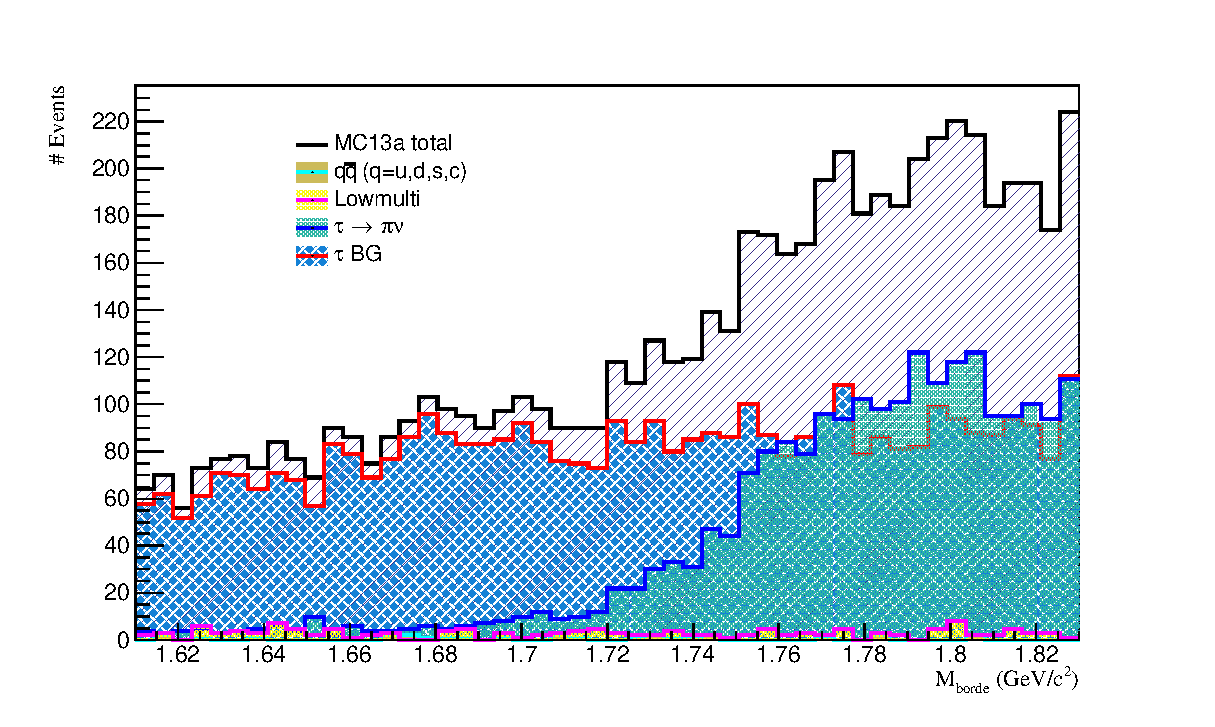
\includegraphics[scale=.6]{Images/m_edge_bdt_fit.eps}
    \caption{\small{Distribución de \(m^{borde}_{\tau}\) MC13a con sus componentes de ruido y señal con corte en BDT>0.2. Distribución en la región de ajuste.}}
    \label{fig:mEdgeFitBdtAllFit}
\end{figure} 


\chapter{Gráficos referentes a la variable \texorpdfstring{$M_{min}$}{TEXT}}

\begin{figure}[h]
  %\setcapwidth{0.6\textwidth}
  \checkoddpage
  \edef\side{\ifoddpage r\else l\fi}%
  \makebox[\textwidth][\side]{%
    \begin{minipage}[t]{0.56\textwidth}
      \centering
    \subfloat[\centering  ]{{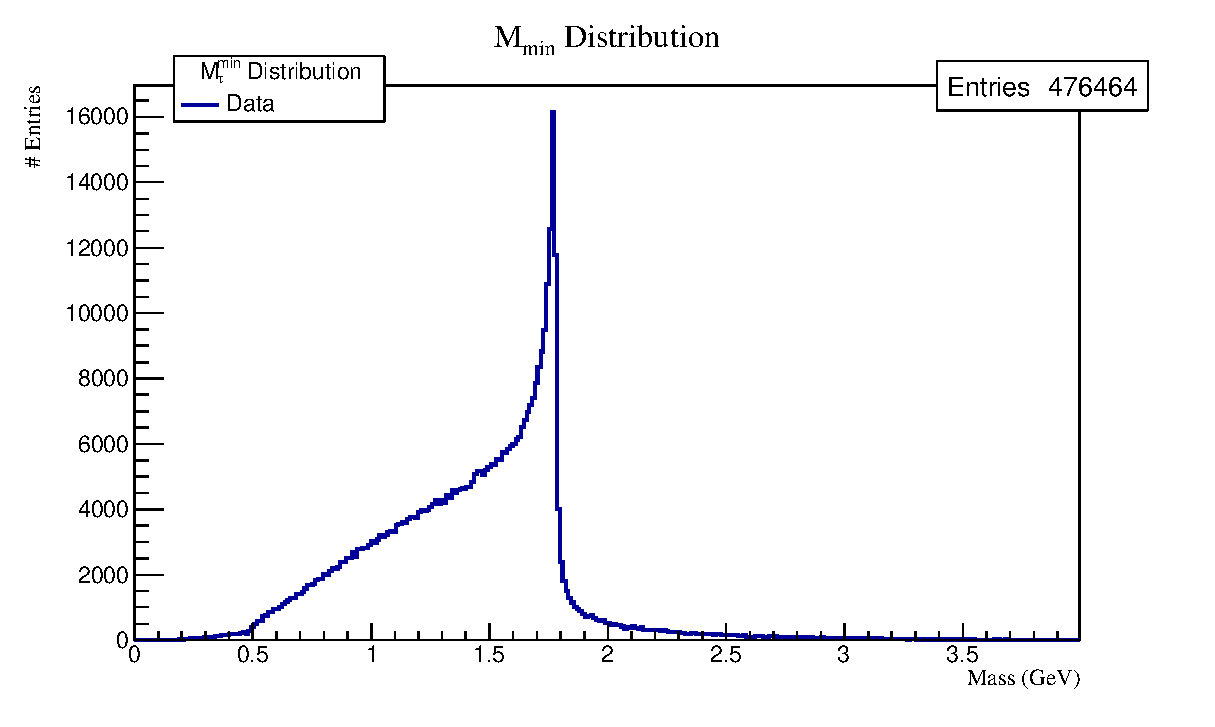
\includegraphics[width=\textwidth]{Images/m_min_complete.eps} }}
      %\caption{Caption 1}
    \end{minipage}%
    \hfill
    \begin{minipage}[t]{0.56\textwidth}
      \centering
    \subfloat[\centering  ]{{\includegraphics[width=\textwidth]{Images/m_min_fit_complete.eps} }}
      %\caption{Caption 2}
    \end{minipage}%
  }%
  \caption{\small{(a) Distribución completa de la variable \(m^{min}_{\tau}\) (sólo señal) de la muestra ``taupair'' de MC13a del experimento Belle II. (b) Distribución de la variable \(m^{min}_{\tau}\) en la región de ajuste.}}
  \label{fig:mMinDistri}
\end{figure}

\begin{figure}[h]
    \centering
    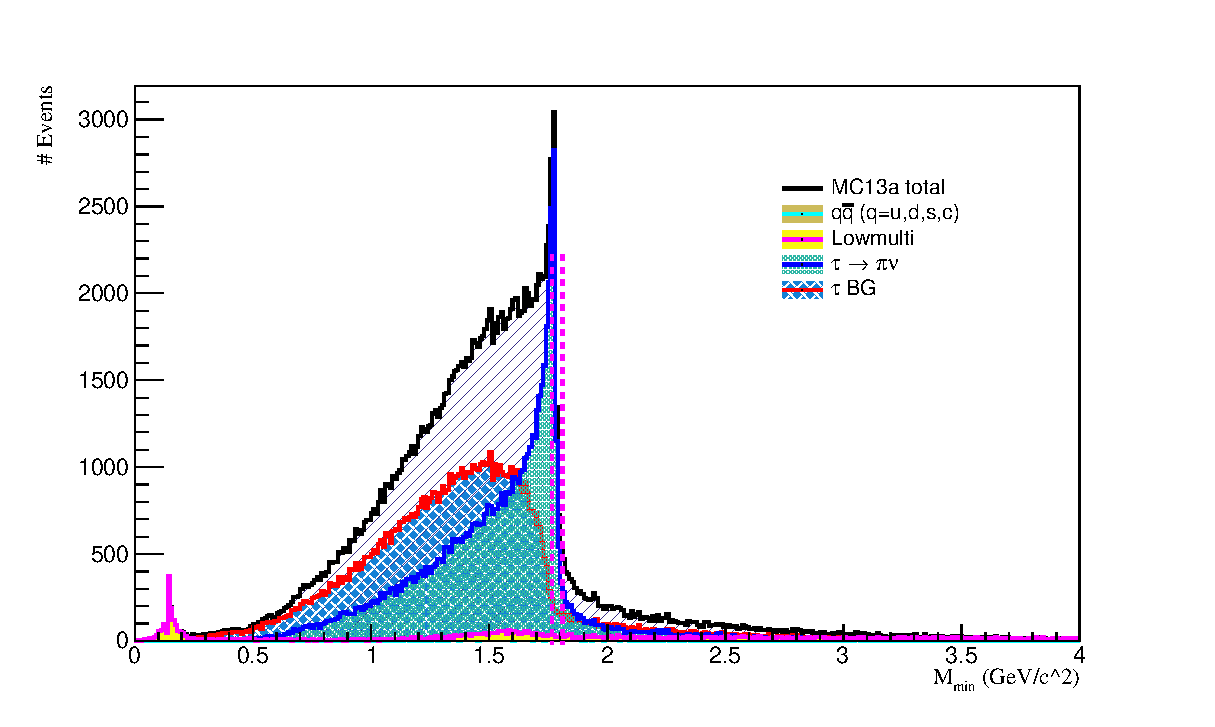
\includegraphics[scale=.6]{Images/m_min_plot_all.eps}
    \caption{\small{Distribución de \(m^{min}_{\tau}\) MC13a con sus componentes de ruido y señal con corte en BDT>0.2. Distribución completa}}
    \label{fig:mMinBdtAll}
\end{figure} 
\begin{figure}[h]
    \centering
    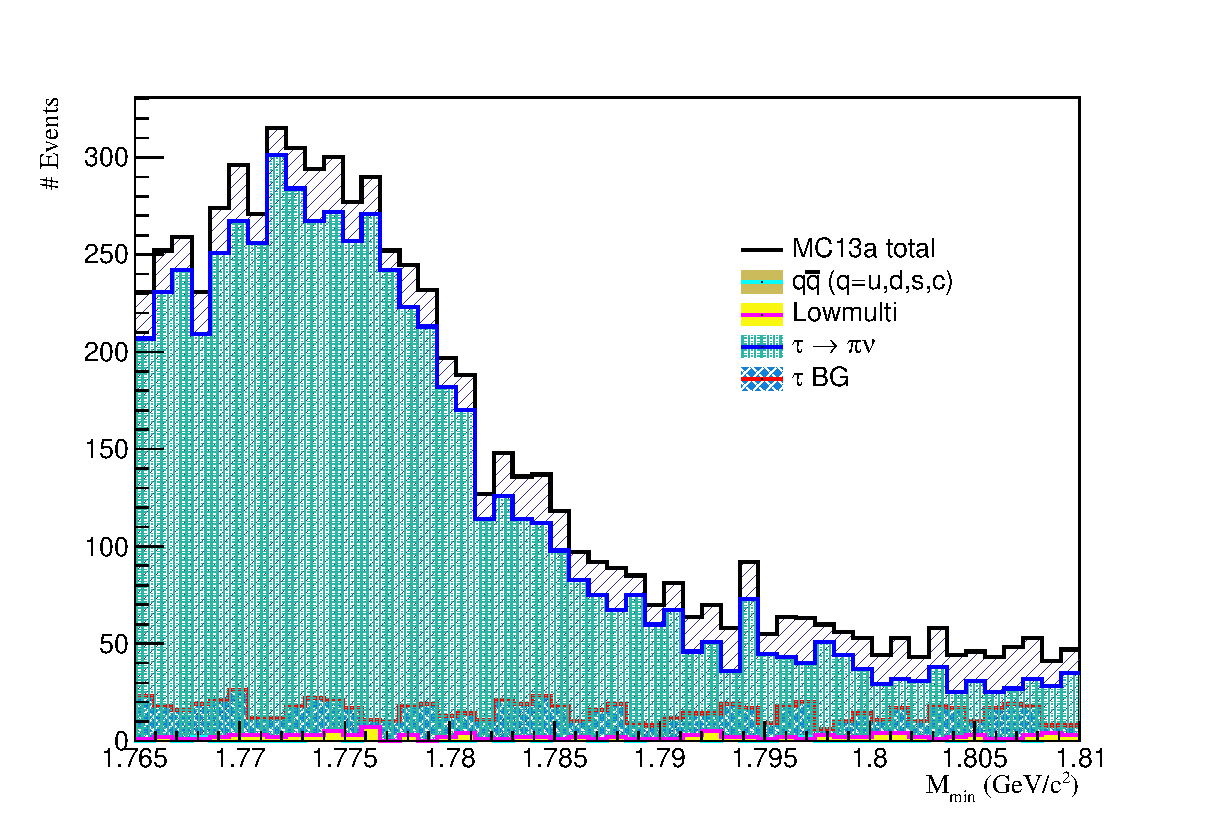
\includegraphics[scale=.6]{Images/m_min_fit_plot.eps}
    \caption{\small{Distribución de \(m^{min}_{\tau}\) MC13a con sus componentes de ruido y señal con corte en BDT>0.2. Distribución en la región de ajuste.}}
    \label{fig:mMinBdtAllFit}
\end{figure} 

 

\chapter{Gráficos referentes a la variable \texorpdfstring{$M_{max}$}{TEXT}}

\begin{figure}[h]
  %\setcapwidth{0.6\textwidth}
  \checkoddpage
  \edef\side{\ifoddpage r\else l\fi}%
  \makebox[\textwidth][\side]{%
    \begin{minipage}[t]{0.56\textwidth}
      \centering
    \subfloat[\centering  ]{{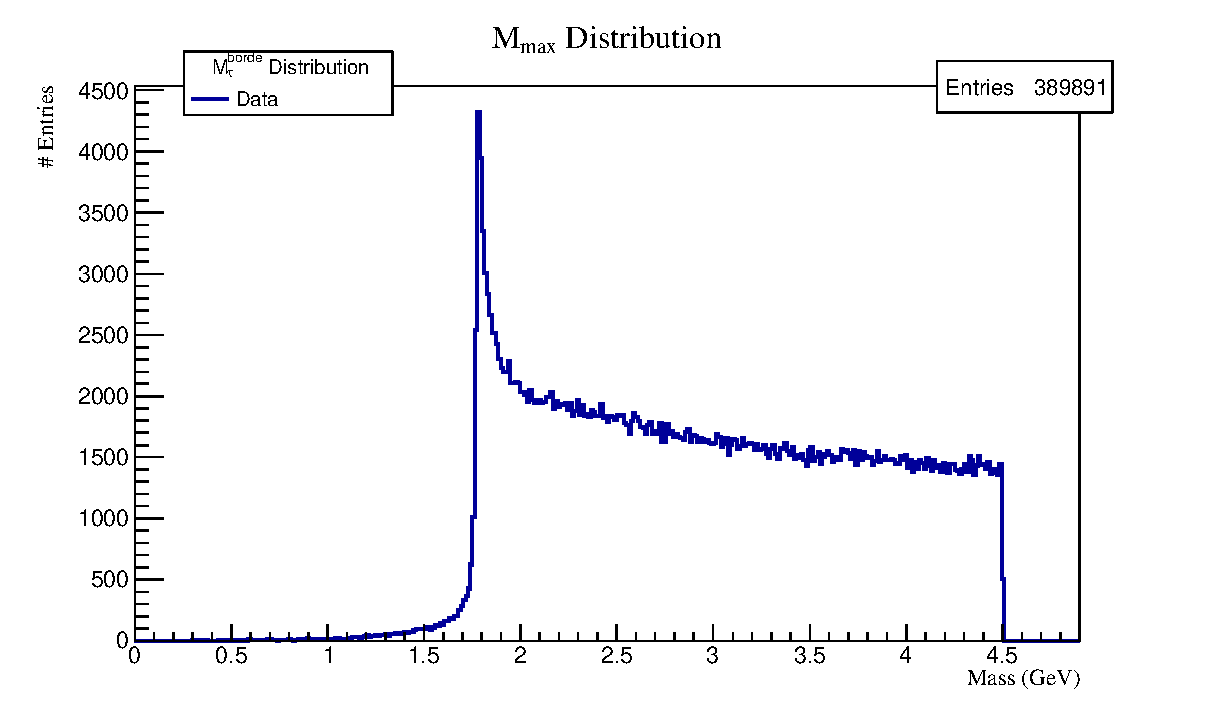
\includegraphics[width=\textwidth]{Images/m_max_distri.eps} }}
      %\caption{Caption 1}
    \end{minipage}%
    \hfill
    \begin{minipage}[t]{0.56\textwidth}
      \centering
    \subfloat[\centering  ]{{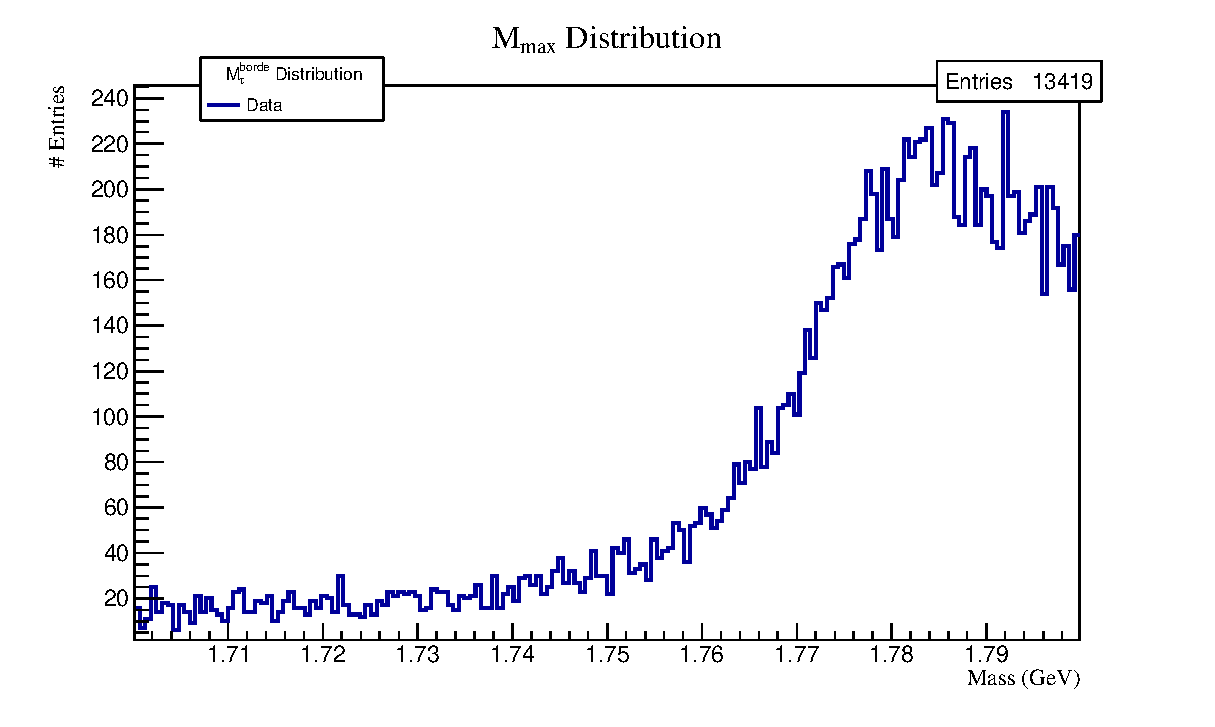
\includegraphics[width=\textwidth]{Images/m_max_distri_fit.eps} }}
      %\caption{Caption 2}
    \end{minipage}%
  }%
  \caption{\small{(a) Distribución completa de la variable \(m^{max}_{\tau}\) (sólo señal) de la muestra ``taupair'' de MC13a del experimento Belle II. (b) Distribución de la variable \(m^{max}_{\tau}\) en la región de ajuste.}}
  \label{fig:mMaxDistri}
\end{figure}
\begin{figure}[h]
    \centering
    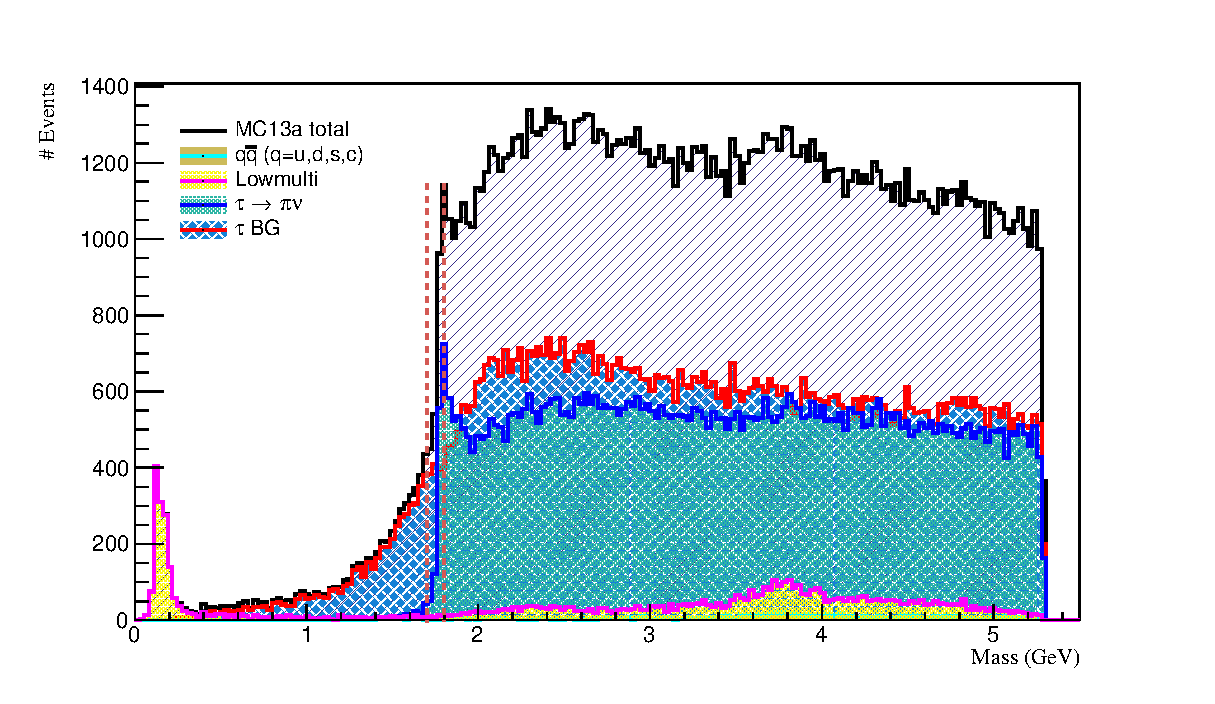
\includegraphics[scale=.6]{Images/m_max_plot_all.eps}
    \caption{\small{Distribución de \(m^{max}_{\tau}\) MC13a con sus componentes de ruido y señal con corte en BDT>0.2. Distribución completa}}
    \label{fig:mMaxBdtAll}
\end{figure} 
\begin{figure}[h]
    \centering
    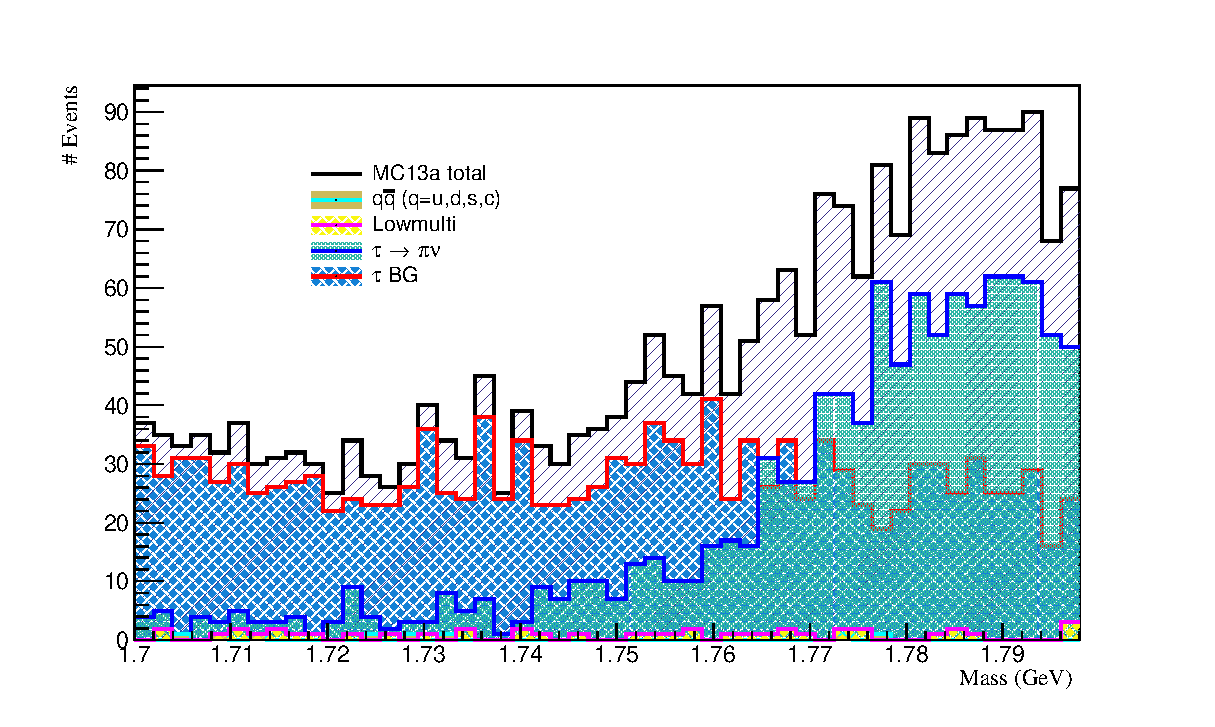
\includegraphics[scale=.6]{Images/m_max_fit_plot.eps}
    \caption{\small{Distribución de \(m^{max}_{\tau}\) MC13a con sus componentes de ruido y señal con corte en BDT>0.2. Distribución en la región de ajuste.}}
    \label{fig:mMaxBdtAllFit}
\end{figure} 

\end{appendices}



%\bibliography{References/sample.bib}
%\include{References}
%\bibliographystyle{apacite}
%\bibliography{sample}
\printbibliography{}
\end{document}
